\documentclass{beamer}

\mode<presentation> {
\usetheme{Madrid}
}

\usepackage{graphicx}
\usepackage{booktabs}
\usepackage[export]{adjustbox}
\graphicspath{{./images/}}
\usepackage{amsmath}

%------------------------------------------------

\title[NMF]{Nonnegative Matrix Factorization (NMF)}

\author{Bernard Lampe and Adam Bekit}
\date{May 5, 2016}

\begin{document}
%------------------------------------------------
\begin{frame}
\titlepage
\end{frame}

%------------------------------------------------
\begin{frame}
\frametitle{Overview}
\begin{columns}

\begin{column}{0.3\textwidth}
\tableofcontents
\end{column}

\begin{column}{0.7\textwidth}
\begin{figure}
  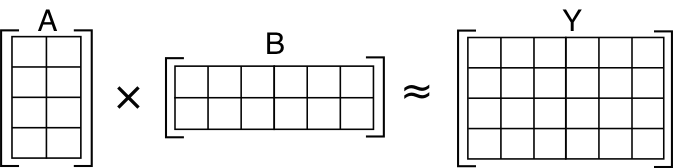
\includegraphics[width=8cm,center]{NMF}
\end{figure}
\end{column}
\end{columns}

\end{frame}

%------------------------------------------------
\section{Theory}
\subsection{Model}
\subsection{Cost Function}
\subsection{Uniqueness}
\subsection{Algorithms}
\subsection{Performance}
\subsection{Diversity}

\section{Application}
\subsection{Description}

\section{Results}
\section{References}

%------------------------------------------------
\begin{frame}
\frametitle{NMF Model}
\begin{align*}
\mathbf{Y} = \mathbf{A}\mathbf{B} + \mathbf{E}, \ \mathbf{Y}  \in \mathbb{R}^{M \times N}, \mathbf{A}  \in \mathbb{R}^{M \times R}, \mathbf{B}  \in \mathbb{R}^{R \times N}
\end{align*}
\begin{align*}
Y_{ij} \approx \sum_{r=1}^{R} A_{ir} B_{rj} 
\end{align*}

\begin{itemize}
\item  $\mathbf{Y}$ is a nonnegative data matrix
\item  $\mathbf{A}$ and $\mathbf{B}$ are nonnegative factor matrices
\item  $\mathbf{E}$ is an error matrix
\item  $\{\mathbf{a}_i\}$, columns of $\mathbf{A}$ are the basis vectors
\item  $\{\mathbf{b}_j\}$, columns of $\mathbf{B}$ are the coordinate vectors
\end{itemize}
\end{frame}

%------------------------------------------------
\begin{frame}
\frametitle{Model Constraints of PCA, VQ, NMF, Dictionary Learning}

Different algorithms can be viewed as matrix decompositions with different constraints on \(\mathbf{A}\) and \(\mathbf{B}\).

\begin{itemize}
\item VQ require $\{\mathbf{a}_i\}$ to be quantized vectors, and $\{\mathbf{b}_{j}\}$ to be unitary 
    \begin{itemize}
        \item $\{\mathbf{a}_i\}$ are the centroids of the K-means algorithm
    \end{itemize}
\item PCA $\{\mathbf{a}_{i}\}$ are orthonormal, and $\mathbf{a}_{1} = \arg\max_{\|\mathbf{a}_{1}\|} { \text{E}\{{\mathbf{a}_1^T\mathbf{y}_i}^2\}, \ \ \  \forall{i}}$
    \begin{itemize}
        \item $\{\mathbf{a}_i\}$ are the eigenvectors of the correlation matrix
    \end{itemize}
\item NMF requires specification of $R$, and that $A_{ij} \ge 0$ and $B_{ij} \ge 0$
\item Dictionary learning requires specification of $R$, and $A_{ij} \in \mathbb{R}$ and $B_{ij} \in \mathbb{R}$
\end{itemize}
\end{frame}

%------------------------------------------------
\begin{frame}
\frametitle{Model Expressiveness}
\begin{itemize}
\item PCA and ICA can add and subtract basis matrix vectors
\item NMF can only add basis matrix vectors leading to ``parts based" models
\item NN-KSVD and non-negative dictionary learning are specific NMF factorizations
\end{itemize}
\end{frame}

%------------------------------------------------
\begin{frame}
\frametitle{PCA, VQ and NMF Examples}
\begin{columns}
\begin{column}{0.5\textwidth}
\begin{figure}[h]
  \vspace*{-1cm}
  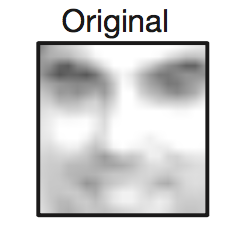
\includegraphics[width=2cm,center]{face}
  \centering
\end{figure}
\end{column}

\begin{column}{0.5\textwidth}
\begin{figure}[h]
  \vspace*{-1cm}
  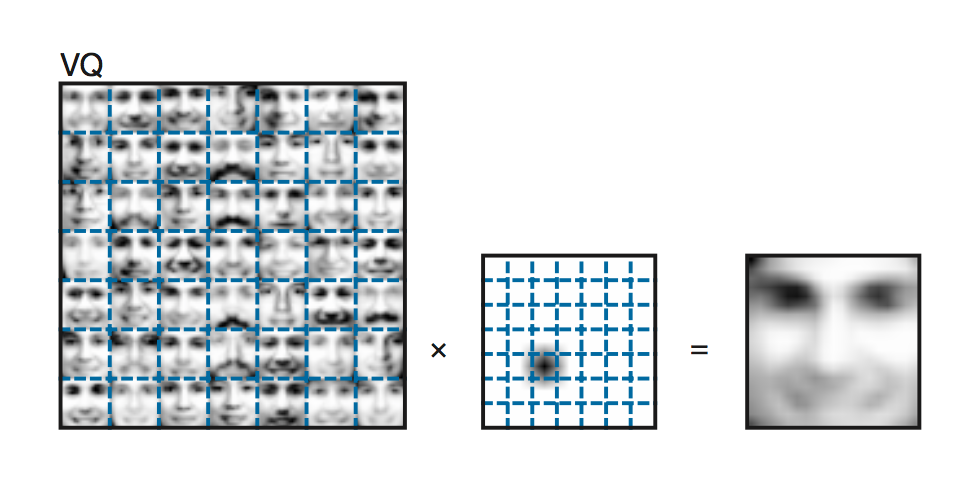
\includegraphics[width=6cm,center]{lee2}
  \centering
\end{figure}
\end{column}
\end{columns}

\begin{columns}
\begin{column}{0.5\textwidth}
\begin{figure}[h]
  \vspace*{-0.5cm}
  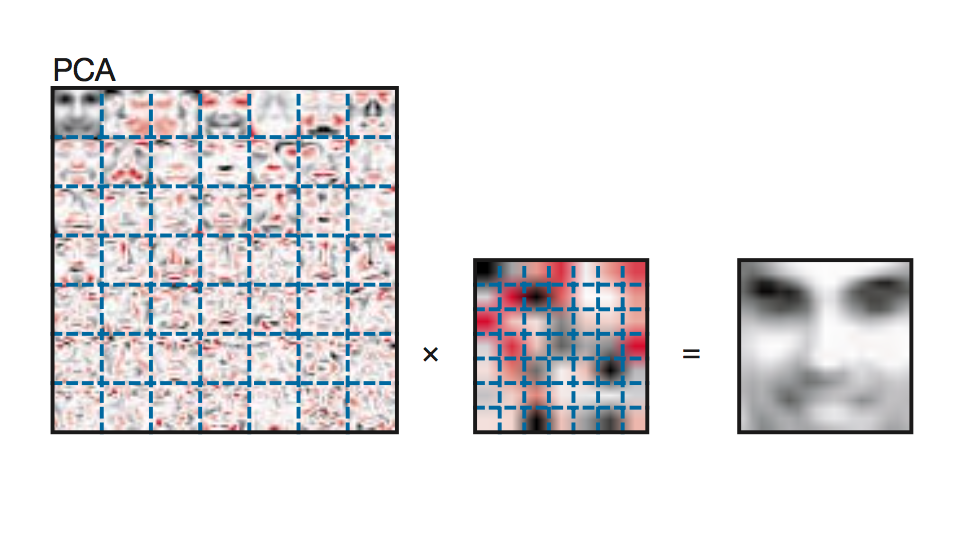
\includegraphics[width=6cm,center]{lee3}
  \centering
\end{figure}
\end{column}

\begin{column}{0.5\textwidth}
\begin{figure}[h]
  \vspace*{-0.5cm}
  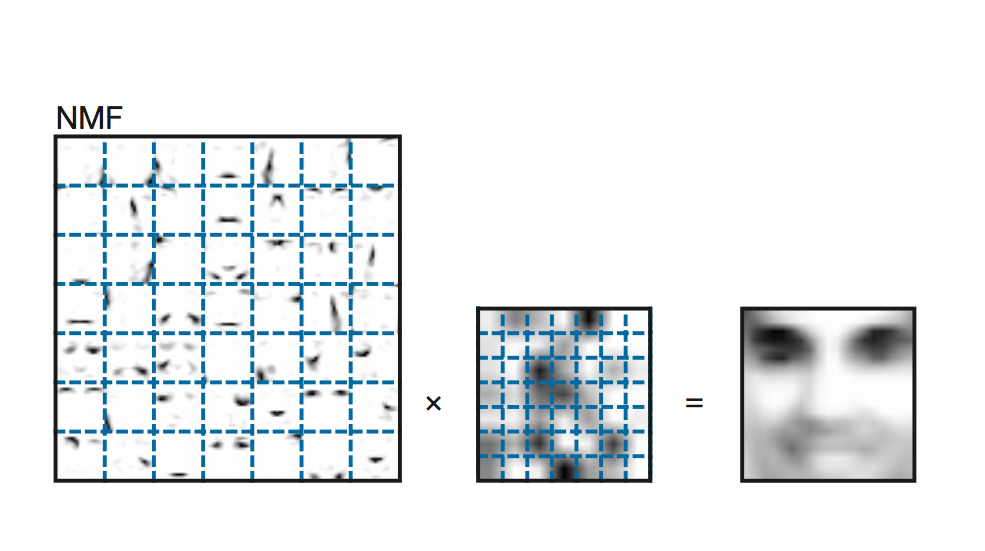
\includegraphics[width=6cm,center]{lee1}
  \centering
\end{figure}
\end{column}
\end{columns}
Basis matricies were trained with 2429, 19x19 pixel face images. [Lee and Seung '99]
\end{frame}

%------------------------------------------------
\begin{frame}
\frametitle{NMF With Sparsity Example}
\begin{figure}[h]
  \centering
  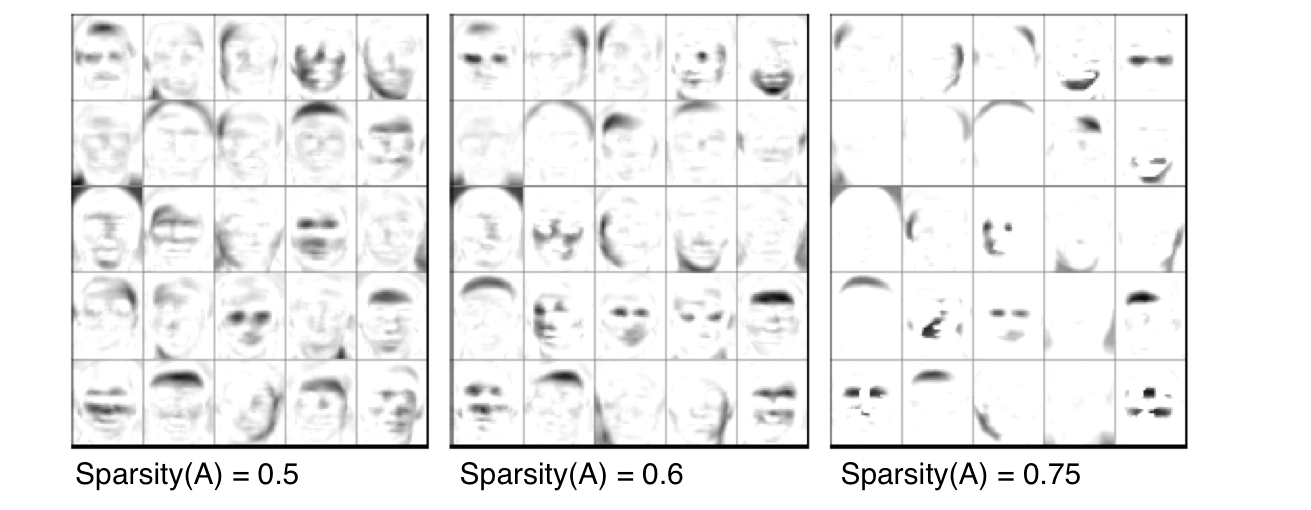
\includegraphics[width=12cm,center]{hoyer}
\end{figure}
[Hoyer '04]
\end{frame}

%------------------------------------------------
\begin{frame}
\frametitle{Model Expressiveness Examples}
\begin{figure}
  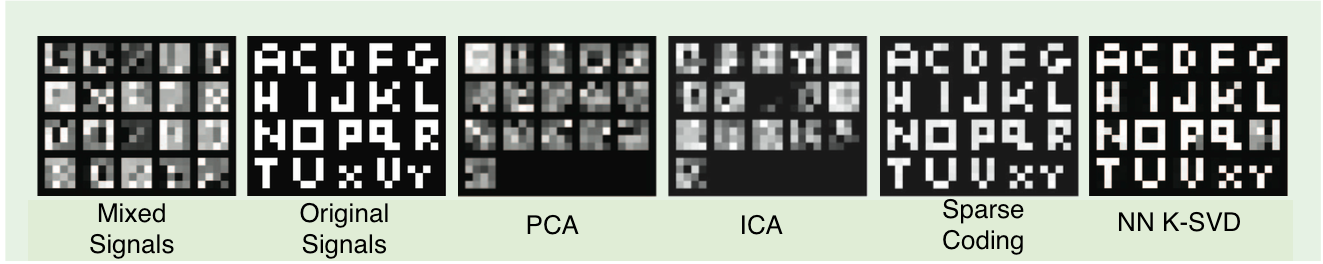
\includegraphics[width=13cm,center]{nnmf_examples}
\end{figure}
[Ivana Tosic and Pascal Frossard '11]

\begin{itemize}
\item VQ, PCA and ICA have linearly independent vectors in the basis matrix
\item PCA and ICA require $R \le \min\{M, N\}$
\item NMF can have linearly dependent vectors in the basis matrix
\end{itemize}
\end{frame}

%------------------------------------------------
\begin{frame}
\frametitle{NMF as K-Means Clustering}

\vspace*{-1cm}
\begin{align*}
J_{\text{K-means}} &= \sum_{i=1}^{n}{\min_{1\le r \le R}{\|\mathbf{y}_i-\mathbf{c}_r\|_F^2}} = \sum_{r=1}^R \sum_{i \in C_r} \|\mathbf{y}_i - \mathbf{c}_r\|_F^2 \\
&= \sum_{i=1}^{n}\sum_{r=1}^{R}{h_{ir}\|\mathbf{y}_i-\mathbf{c}_r\|_F^2} = \|\mathbf{Y} - \mathbf{A}\mathbf{B}\|_F^2 = J_{nmf}
\end{align*}

\begin{align*}
\mathbf{c}_r = \frac{1}{|C_r|}\sum_{i \in C_r}{\mathbf{y}_i}, \ \ \ \mathbf{y}_i \in C_r, \ \ \ h_{ir} = \{0,1\}
\end{align*}

\begin{itemize}
\item NMF can be considered a clustering of the data into $R$ clusters with $\{\mathbf{a}_i\}$ centroids and $\{\mathbf{b}_j\}$ being unitary [C. Ding, et al '05]
\item The centroids do not necessarily have to be positive, therefore this is refered to as ``semi-NMF" or ``relaxed-NMF"
\end{itemize}

\end{frame}

%------------------------------------------------
\begin{frame}
\frametitle{NMF as Probabilistic Latent Variables}
\begin{figure}
  \vspace*{-1cm}
  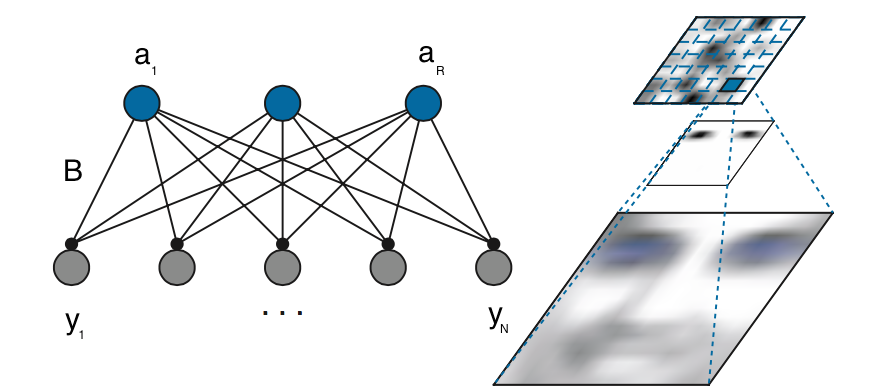
\includegraphics[width=8cm,center]{lee4}
\end{figure}

\begin{itemize}
\item Visible units $\{\mathbf{y}_i\}$ are connected to hidden latent variables $\{\mathbf{a}_j\}$ through weights in $\mathbf{B}$
\item If $\{\mathbf{b}_j\}$ are normal, then $\{\mathbf{b}_j\}$ can be viewed as probability distributions
\item If $J_{nmf} = D_{KL}(\mathbf{Y}\|\mathbf{A}\mathbf{B})$, then the problem is exactly probabilistic latent semantic analysis [C.Ding '08]
\end{itemize}
\end{frame}


%------------------------------------------------
\begin{frame}
\frametitle{Cost Functions}
NMF is implemented by minimizing a non-convex cost function
\begin{itemize}
\item Euclidean Distance Minimization
	\begin{align*} 
		J_{\text{nmf}}^* = \arg\min_{\mathbf{A,B}} {\frac{1}{2}||\mathbf{Y} - \mathbf{A} \mathbf{B}||}_{2}^2  \ \ \    \text{s.t.} \ \ \ \mathbf{A}, \mathbf{B}  \ge 0
	\end{align*}
\item Frobenius  Distance Minimization
	\begin{align*} 
		J_{\text{nmf}}^* = \arg\min_{\mathbf{A,B}} {\frac{1}{2}||\mathbf{Y} - \mathbf{A} \mathbf{B}||}_{F}^2  \ \ \    \text{s.t.} \ \ \ \mathbf{A}, \mathbf{B}  \ge 0
	\end{align*}
\item K-L Distance Minimization
	\begin{align*} 
		J_{\text{nmf}}^* = \arg\min_{\mathbf{A,B}} { D_{KL}(\mathbf{Y}\|\mathbf{A}\mathbf{B}) } = \arg\min_{\mathbf{A,B}} { \sum_{ij}(Y_{ij}\text{log}{\frac{Y_{ij}}{[\mathbf{A}\mathbf{B}]_{ij}} - Y_{ij} + {[\mathbf{A}\mathbf{B}}]_{ij})}}
	\end{align*}
\end{itemize}

%------------------------------------------------
\end{frame}

\begin{frame}
\frametitle{Uniqueness}
Factorization is not unique
\begin{align*}
\mathbf{Y} \approx (\mathbf{A} \mathbf{T}) (\mathbf{T}^{-1} \mathbf{B}) = \mathbf{A}' \mathbf{B}'
\end{align*}

We can enforce a unique solution by including regularization (i.e., sparsity)
	\begin{align*} 
		J_{\text{nmf}}^* = \arg\min_{\mathbf{A,B}} {\frac{1}{2}||\mathbf{Y} - \mathbf{A} \mathbf{B}||}_{2}^2 + \lambda_0 \|A\|_0 + \lambda_1 \|B\|_0 \ \ \    \text{s.t.} \ \ \ \mathbf{A}, \mathbf{B}  \ge 0
	\end{align*}

If the sparsity of the \(\mathbf{A}\) or \(\mathbf{B}\) is low enough, then the solution is unique

\begin{align*}
\|\mathbf{B}\|_0 < \frac{R\ \text{spark}(\mathbf{A})}{2} \ \ \ \text{ [Donoho and Elad '02]}
\end{align*}

Spark is the smallest number of columns that are linearly dependent
\begin{align*}
\text{spark}(\mathbf{A}) = \min_{\mathbf{d} \ne 0}\|\mathbf{d}\|_0  \ \ \ \text{s.t.} \ \ \ \mathbf{A}\mathbf{d} = \mathbf{0}
\end{align*}

\end{frame}

%------------------------------------------------
\begin{frame}
\frametitle{Algorithms Used in Project}
Optimization algorithms for NMF non-convex cost functions

\begin{itemize}
	\item Alternating Least Squares (ALS)
		\begin{itemize}
			\item $J_{\text{nmf}}$ is minimized by alternating between $\mathbf{A}$ and $\mathbf{B}$
			\item $J_{\text{nmf}}$ is minimized while holding $\mathbf{A}$ fixed and minimizing $\mathbf{B}$ and vise versa
		\end{itemize}
	\item Multiplicative Update (MU)
		\begin{itemize}
			\item $J_{\text{nmf}}$ is minimized by fixing $\mathbf{A}$ and $\mathbf{B}$
			\item $\mathbf{A}$ and $\mathbf{B}$ are updated using a multiplicative update rule
		\end{itemize}
	\item Hierarchical Alternating Least Squares (HALS)
		\begin{itemize}
			\item $J_{\text{nmf}}$ is minimized by fixing $\mathbf{A}$ and $\mathbf{B}$
			\item Only one column of $\mathbf{A}$ or $\mathbf{B}$ is updated using an update rule
		\end{itemize}
	\item Multiplicative Update (MU) with Sparsity Constraint
		\begin{itemize}
			\item $J_{\text{nmf}}$ is minimized by fixing $\mathbf{A}$ and $\mathbf{B}$
			\item $\mathbf{A}$ and $\mathbf{B}$ are updated using a sparse multiplicative update rule
		\end{itemize}
	\end{itemize}	
\end{frame}

\begin{frame}
\frametitle{Alternating Least Squares Optimization}

	\begin{align*} 
		J_{\text{nmf}} = \arg\min_{\mathbf{A,B}} {\frac{1}{2}||\mathbf{Y} - \mathbf{A} \mathbf{B}||}_{2}^2  \ \ \    \text{s.t.} \ \ \ \mathbf{A}, \mathbf{B}  \ge 0
	\end{align*}
	
\begin{table}[h]
      \label{tab:ALS} 
\centering
  \begin{tabular}{c || c |  }
        \hline
              & Algorithm: Alternating Least Squares (ALS)\\ \hline \hline
    1: & Initialize  $\mathbf{A}$  and $\mathbf{B}$  \\ \hline
    2: & $\textbf{Repeat}$ \\ \hline
    3: &     solve: $\arg\min_{\mathbf{B}} {\frac{1}{2}||\mathbf{Y} - \mathbf{A} \mathbf{B}||}_{2}^2  \ \ \    \text{s.t.} \ \ \ \mathbf{A}, \mathbf{B}  \ge 0 $ \\  \hline
    4: &     solve: $\arg\min_{\mathbf{A}} {\frac{1}{2}||\mathbf{Y} - \mathbf{A} \mathbf{B}||}_{2}^2  \ \ \    \text{s.t.} \ \ \ \mathbf{A}, \mathbf{B}  \ge 0 $ \\  \hline
    5: & $\textbf{Stopping Condition}$ \\ \hline
    \hline
  \end{tabular}
\end{table}
[Paatero and Tapper '94]

\end{frame}

\begin{frame}
\frametitle{Multiplicative Update Optimization}

	\begin{align*} 
		J_{\text{nmf}} = \arg\min_{\mathbf{A,B}} {\frac{1}{2}||\mathbf{Y} - \mathbf{A} \mathbf{B}||}_{2}^2  \ \ \    \text{s.t.} \ \ \ \mathbf{A}, \mathbf{B}  \ge 0
	\end{align*}
	
\begin{table}[h]
      \label{tab:MU} 
\centering
  \begin{tabular}{c || c |  }
        \hline
              & Algorithm: Multiplicative Update (MU) \\ \hline \hline
    1: & Initialize  $\mathbf{A}^0$, $\mathbf{B}^0$, k = 0  \\ \hline
    2: & $\textbf{Repeat}$ \\ \hline
    3: &     $A_{ir}^{k+1}$=$A_{ir}^k$ $\frac{\left(\mathbf{Y}\mathbf{B}^k\right)_{ir}}{\left(\mathbf{A}^k(\mathbf{B}^k)^T\mathbf{B}^k\right)_{ir}}, \ \ \ 1 \le i \le M, 1 \le r \le R $\\  \hline
    4: &     $B_{rj}^{k+1}$=$B_{rj}^k$ $\frac{\left(\mathbf{Y}^T\mathbf{A}^{k+1}\right)_{rj}}{\left(\mathbf{B}^k(\mathbf{A}^{k+1})^T\mathbf{A}^{k+1}\right)_{rj}}, \ \ \ 1 \le j \le N, 1 \le r \le R$ \\  \hline
    5: &     $k = k + 1$ \\ \hline
    6: & $\textbf{Stopping Condition}$ \\ \hline
    \hline
  \end{tabular}
\end{table}
[Lee and Seung '99]

\end{frame}

%------------------------------------------------
\begin{frame}
\frametitle{HALS / NN-KSVD Optimization}

\begin{table}[h]
      \label{tab:KSVD} 
\centering
  \begin{tabular}{c || c |  }
        \hline
              & Algorithm: HALS / NN-KSVD \\ \hline \hline
    1: & Random Initialization of   $\mathbf{A}^0$, J = 1  \\ \hline
    2: & $\textbf{Repeat}$ \\ \hline
    3: &Use pursuit algorithm to compute  $\{\mathbf{b}_j\}$ \\  \hline
        &      $\arg\min_{\mathbf{B}} {||\mathbf{Y}_{i} - \mathbf{A} \mathbf{B}||}_{2}^2 \ \ \| \mathbf{b}\|_0  \le T_0$ \\  \hline
    4: & Update Stage: For k = 1, 2, \dots , R  \\  \hline   
        & Define group that use $ \{\mathbf{a}_k\}: w_k, i \in N,   \mathbf{b}_i(k) \neq 0$ \\  \hline
        & Compute: $\mathbf{E}_k=\mathbf{Y}-(\mathbf{AB}- \mathbf{a}_k (\mathbf{b}^k)^T)$ \\  \hline
        & Restrict $\mathbf{E}_k$, choose only columns corresponding to $w_k$, get $\mathbf{E}_k^{w_k}$ \\  \hline
        & Apply SVD, $\mathbf{E}_k^{w_k}=\mathbf{U} \Delta \mathbf{V}^T, \ \  \mathbf{a}_k= \mathbf{u}_1, \ \  \mathbf{b}^k= \Delta (1,1)   \mathbf{v}_1$    \\  \hline
    5: &     $J = J + 1$ \\ \hline
    6: & $\textbf{Stopping Condition}$ \\ \hline
    \hline
  \end{tabular}
\end{table}

[Michal Aharon, et al '06]

\end{frame}

%------------------------------------------------
\begin{frame}
\frametitle{Multiplicative Update With Sparsity Optimization}

	\begin{align*} 
		J_{\text{nmf}} = \arg\min_{\mathbf{A,B}} {\frac{1}{2}||\mathbf{Y} - \mathbf{A} \mathbf{B}||}_{2}^2  \ \ \    \text{s.t.} \ \ \ \mathbf{A}, \mathbf{B} \ge 0,\ S(\mathbf{a}_i) = S_a,\ S(\mathbf{b}_j) = S_b
	\end{align*}

	\begin{align*} 
		S(\mathbf{x}) = \frac{\sqrt{n} - \|\mathbf{x}\|_1 / \|\mathbf{x}\|_2}{\sqrt{n}-1}  \ \ \ \text{s.t.} \ \ \ n = \text{dim}(\mathbf{x})
	\end{align*}
	
	
\begin{table}[h]
      \label{tab:MU} 
\centering
  \begin{tabular}{c || c |  }
        \hline
              & Algorithm: Multiplicative Update with Sparsity (MU) \\ \hline \hline
    1: & Initialize  $\mathbf{A}^0$, $\mathbf{B}^0$, $k = 0$, $\mu_\mathbf{A}$, $\mu_\mathbf{B}$  \\ \hline
    2: & $\textbf{Repeat}$ \\ \hline
    3: &     $\mathbf{A} = \mathbf{A} - \mu_\mathbf{A}(\mathbf{A}\mathbf{B} - \mathbf{Y})\mathbf{B}^T$ \\ \hline
    4: &     project: $\{\mathbf{a}_i\}\ \ \ \text{s.t.} \ \ \ \|\mathbf{a}_i\|_1 = S_a$ \\ \hline
    5: &     $\mathbf{B} = \mathbf{B} - \mu_\mathbf{B}\mathbf{A}^T(\mathbf{A}\mathbf{B} - \mathbf{Y})$ \\ \hline
    6: &     project: $\{\mathbf{b}_j\}\ \ \ \text{s.t.} \ \ \ \|\mathbf{b}_j\|_1 = S_b$ \\ \hline
    7: & $\textbf{Stopping Condition}$ \\ \hline
    \hline
  \end{tabular}
\end{table}

[Hoyer '04]
\end{frame}

%------------------------------------------------
\begin{frame}
\frametitle{Performance}
Big-O Complexity of NMF Algorithms
\begin{align*}
\mathbf{Y} = \mathbf{A}\mathbf{B} + \mathbf{E}, \ \mathbf{Y}  \in \mathbb{R}^{M \times N}, \mathbf{A}  \in \mathbb{R}^{M \times R}, \mathbf{B}  \in \mathbb{R}^{R \times N}
\end{align*}
\begin{itemize}
\item For R = 1: ``Easy",  [Perron-Frobenius and Eckart-Young theorems '11]
\item Rank($\mathbf{Y}$) = 2: $\text{Rank}_+$($\mathbf{Y}$) = 2, ``Easy"
\item Rank($\mathbf{Y}$) = R: $\mathcal{O}$$((M \times N)^{R^2})$,  [Arora et al. '12, Moitra '13]

\end{itemize}
\begin{table}[h]
      \label{tab:MU} 
\centering
  \begin{tabular}{c || c |  }
        \hline
    Algorithm & Complexity per iteration\\ \hline \hline
    ALS: &  $\mathcal{O}$$(M \times N \times R)$  \\ \hline
    MU:  &  $\mathcal{O}$$(M\times N \times R)$ \\ \hline
    HALS:  &  $\mathcal{O}$$(M\times N \times R)$ \\ \hline
  \end{tabular}
\end{table}
[Guoxu Zhou, et al '14]

\end{frame}

%------------------------------------------------
\begin{frame}
\frametitle{Other Methods}
	\begin{itemize}
		\item Inexact Alternating Least Square (IALS)
		\item Accelerating Proximal Gradient (APG)
		\item Seperable NMF (Sep-NMF)
		\item Squential NMF (Seq-NMF)
        \item Multi-factor NMF (MF-NMF)
        \item NMF Based on Low Rank Approximations
        \item Non-negative Sparse Coding
        \item Many Others...
	\end{itemize}
\end{frame}

%------------------------------------------------
\begin{frame}
\frametitle{Problem Description}
\vspace*{-0.7cm}
\begin{figure}[h]
  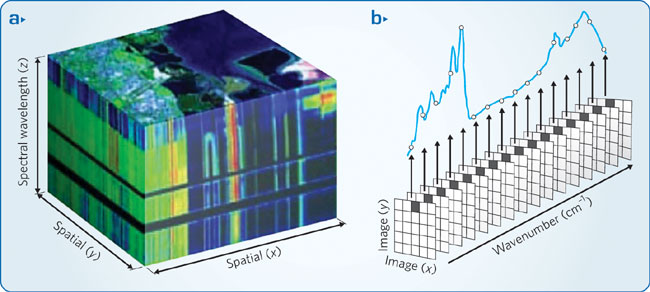
\includegraphics[width=8cm,center]{him}
  \centering
\end{figure}
\vspace*{-0.5cm}
[David Bannon '09]

\begin{itemize}
\item HSI pixels are non-negative
\item Pixels are superpositions of a finite number of materials with non-negative reflectance
\item Applying NMF to solve the unsupervised HSI unmixing problem
\end{itemize}
\end{frame}

%------------------------------------------------
\begin{frame}
\frametitle{Diversity in Hyperspectral Images (HSI)}
\begin{itemize}
\item Minimize mutual coherence between $\{\mathbf{a}_i\}$
    \begin{align*}
        M(\{\mathbf{a}_i\}) = \max_{1 \le i \ne j \le R} { \frac{|\mathbf{a}_i^T\mathbf{a}_j|}{\|\mathbf{a}_i\|_2 \|\mathbf{a}_j\|_2} }
    \end{align*}
\item Minimize sparsity of $\{\mathbf{b}_j\}$
    \begin{align*}
        1 \le \|\mathbf{b}_j\|_0 \le R
    \end{align*}
\end{itemize}

\end{frame}


%------------------------------------------------
\begin{frame}
\frametitle{HSI Decomposition}

\begin{itemize}
\item What are the basis vectors that ``best" represent the image?
\begin{itemize}
\item The material types can be represented by the columns of $\mathbf{A}$
\item You can group and classify pixels from these types
\end{itemize}
\item What are the coefficients for each pixel in the image?
\begin{itemize}
\item The abundance fractions can be represented by the columns of $\mathbf{B}$
\end{itemize}
\item Each pixel in $\mathbf{Y}$ is then represented by a linear combination of $\mathbf{A}$ and columns of $\mathbf{B}$
	\begin{align*}
    Y_{ij} \approx \sum_{r=1}^{R} A_{ir} B_{rj} 
	\end{align*}
\item The error due to approximation is 
	\begin{align*}
	\mathbf{E} = \mathbf{Y}-\mathbf{A}\mathbf{B}
	\end{align*}
\end{itemize}
\end{frame}

%------------------------------------------------
\begin{frame}
\frametitle{Linear Unmixing}

\begin{itemize}
\item What are the basis vectors that ``best" represent the image?
\begin{itemize}
\item The material types can be represented by the columns of $\mathbf{A}$
\item You can group and classify pixels from these types
\end{itemize}
\item What are the coefficients for each pixel in the image?
\begin{itemize}
\item The abundance fractions can be represented by the columns of $\mathbf{B}$
\end{itemize}
\item Each pixel in $\mathbf{Y}$ is then represented by a linear combination of the columns of $\mathbf{A}$
	\begin{align*}
    Y_{ij} \approx \sum_{r=1}^{R} A_{ir} B_{rj} 
	\end{align*}
\end{itemize}
\end{frame}

%------------------------------------------------
\begin{frame}
\frametitle{Collected and Synthetic Data}
\begin{columns}
    \begin{column}{0.5\textwidth}
        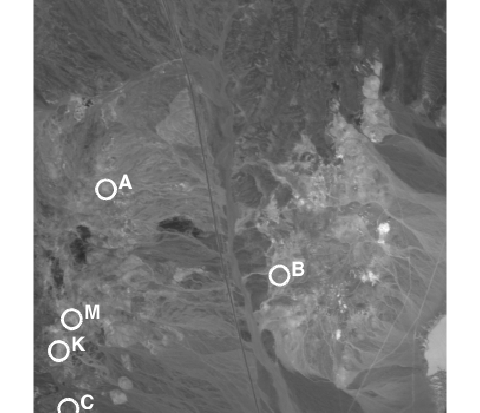
\includegraphics[width=4cm,center]{cuprite_groundTruth}
        \centering
        \\ Cuprite Dimension \(350\)x\(350\)x\(189\)

        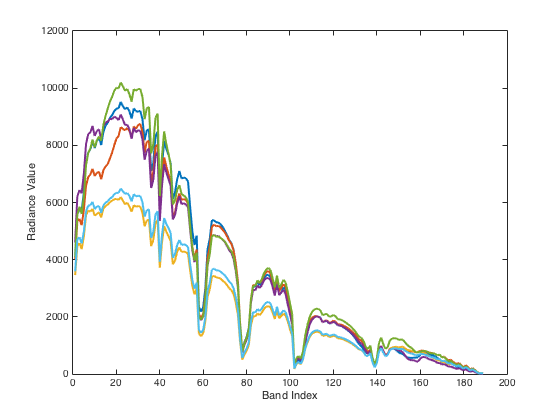
\includegraphics[width=4cm,center]{radiance}
        \centering
        \\ Plots of marked endmembers
    \end{column}
    \begin{column}{0.5\textwidth}
        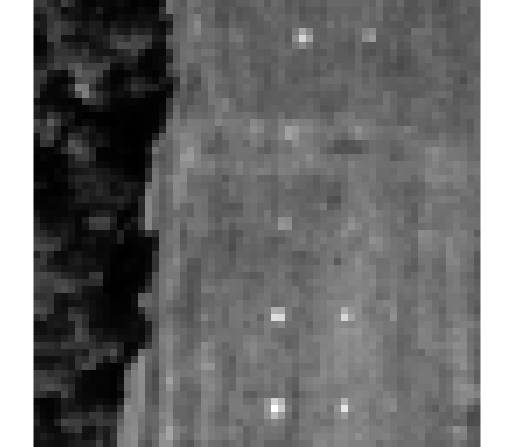
\includegraphics[width=4cm,center]{hydice}
        \centering
        \\ Hydice Dimension \(64\)x\(64\)x\(169\)

        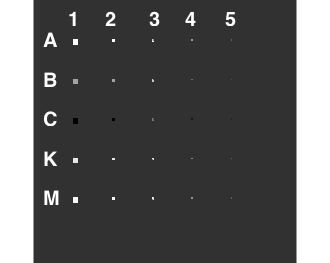
\includegraphics[width=4cm,center]{synthetic_labeled}
        \centering
        \\ Synthetic \(200\)x\(200\)x\(189\)
    \end{column}
\end{columns}
\end{frame}

%------------------------------------------------
\begin{frame}
\frametitle{Numerical Error $\&$ Mutual Coherence}
\begin{columns}
    \begin{column}{0.33\textwidth}
        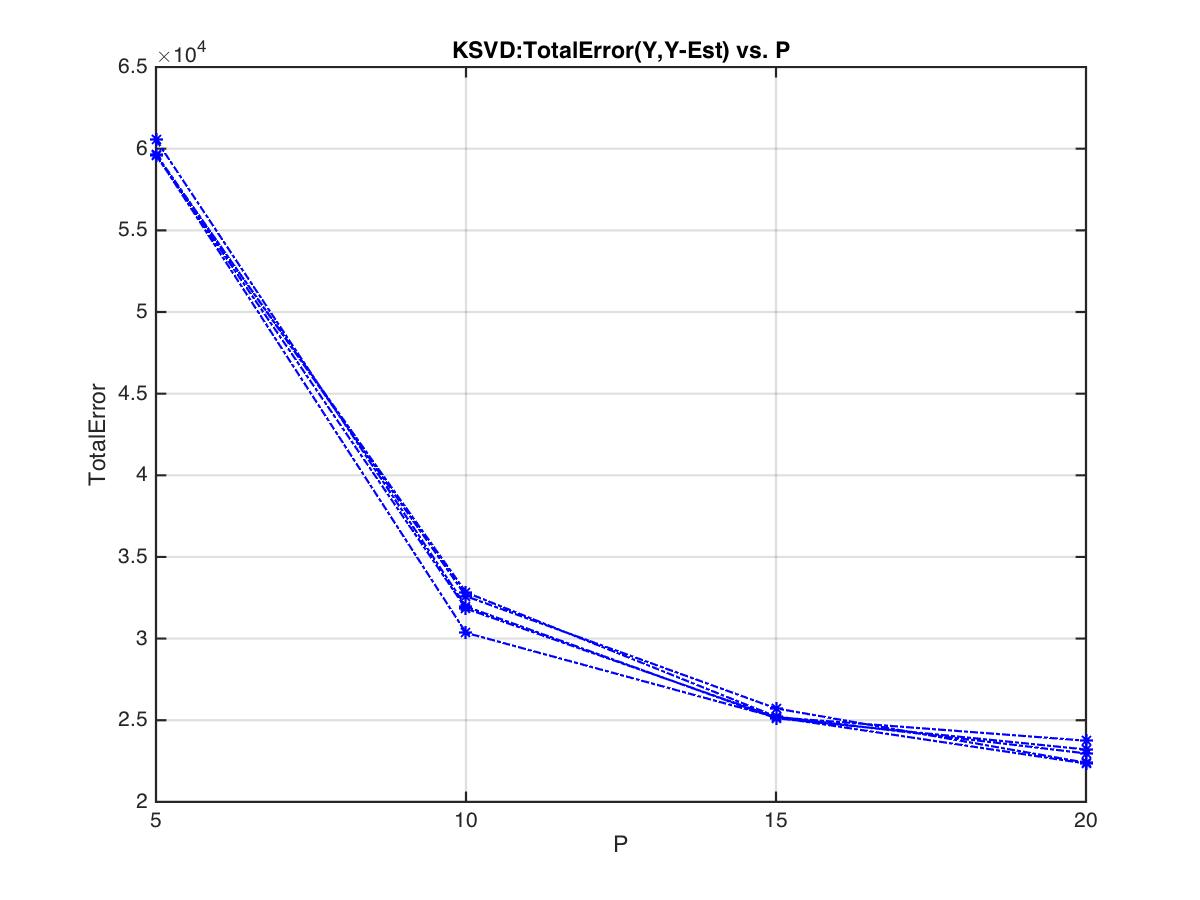
\includegraphics[width=4cm,center]{KSVD_TotalError}
        \\ KSVD Error vs. P
        \centering

        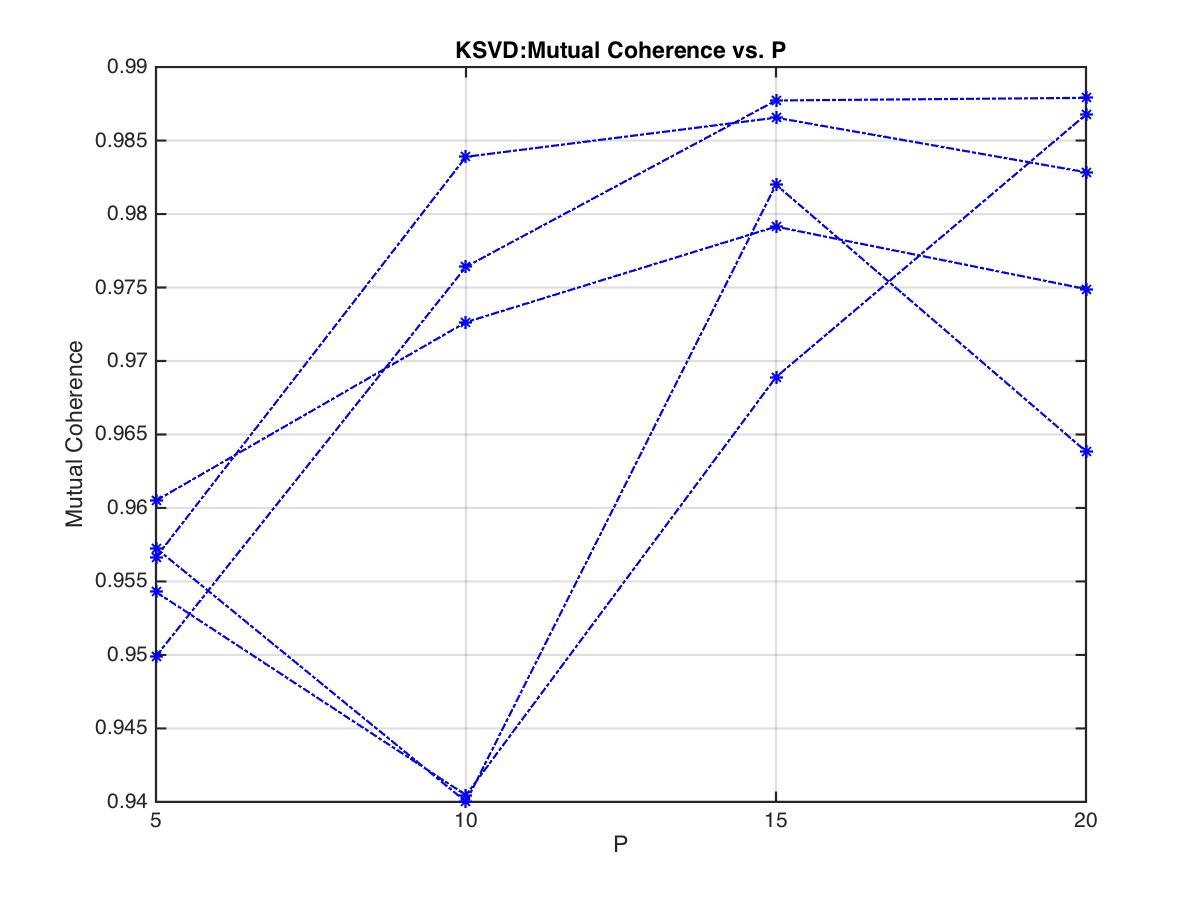
\includegraphics[width=4cm,center]{KSVD_Mutual_Coherence}
        \\ KSVD MC vs. P
        \centering
    \end{column}
    \begin{column}{0.33\textwidth}
        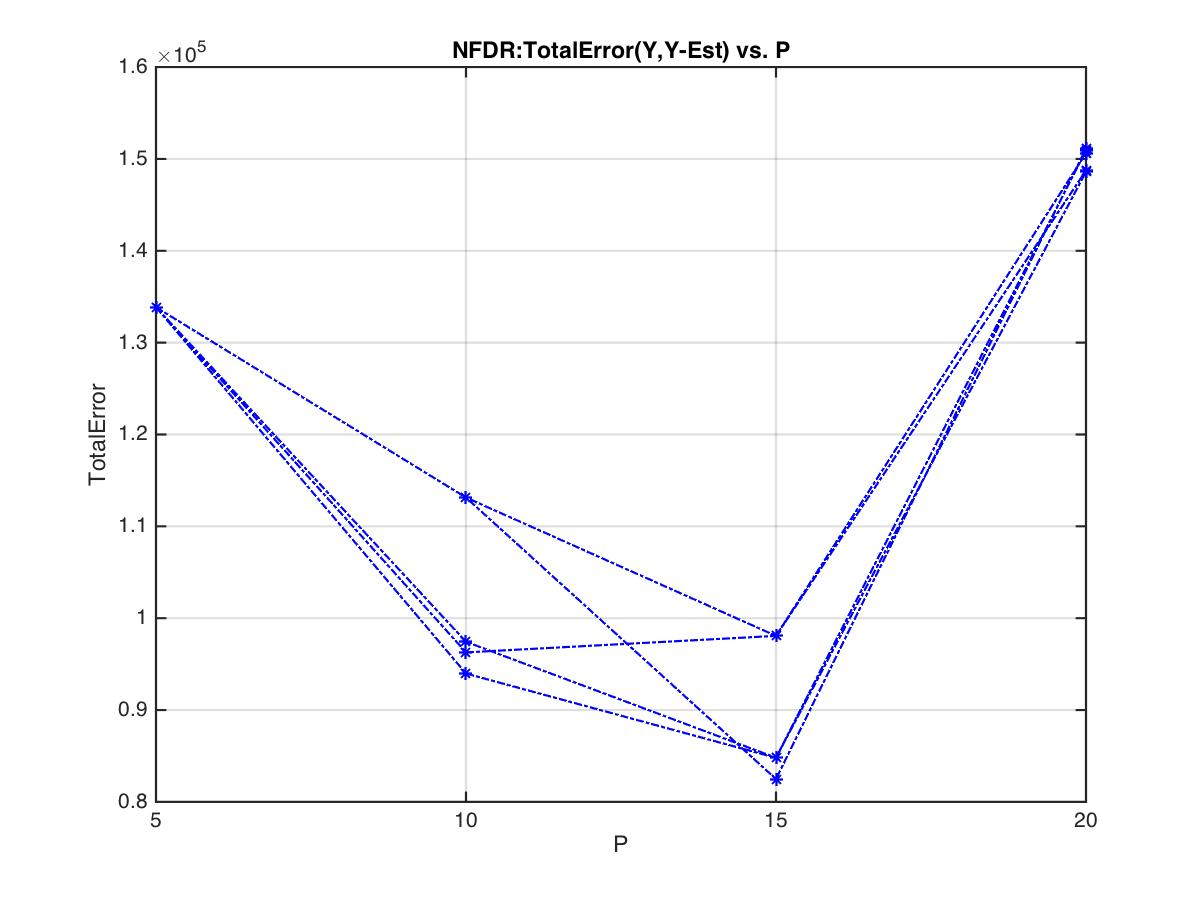
\includegraphics[width=4cm,center]{NFDR_TotalError}
        \\ NFDR Error vs. P
        \centering

        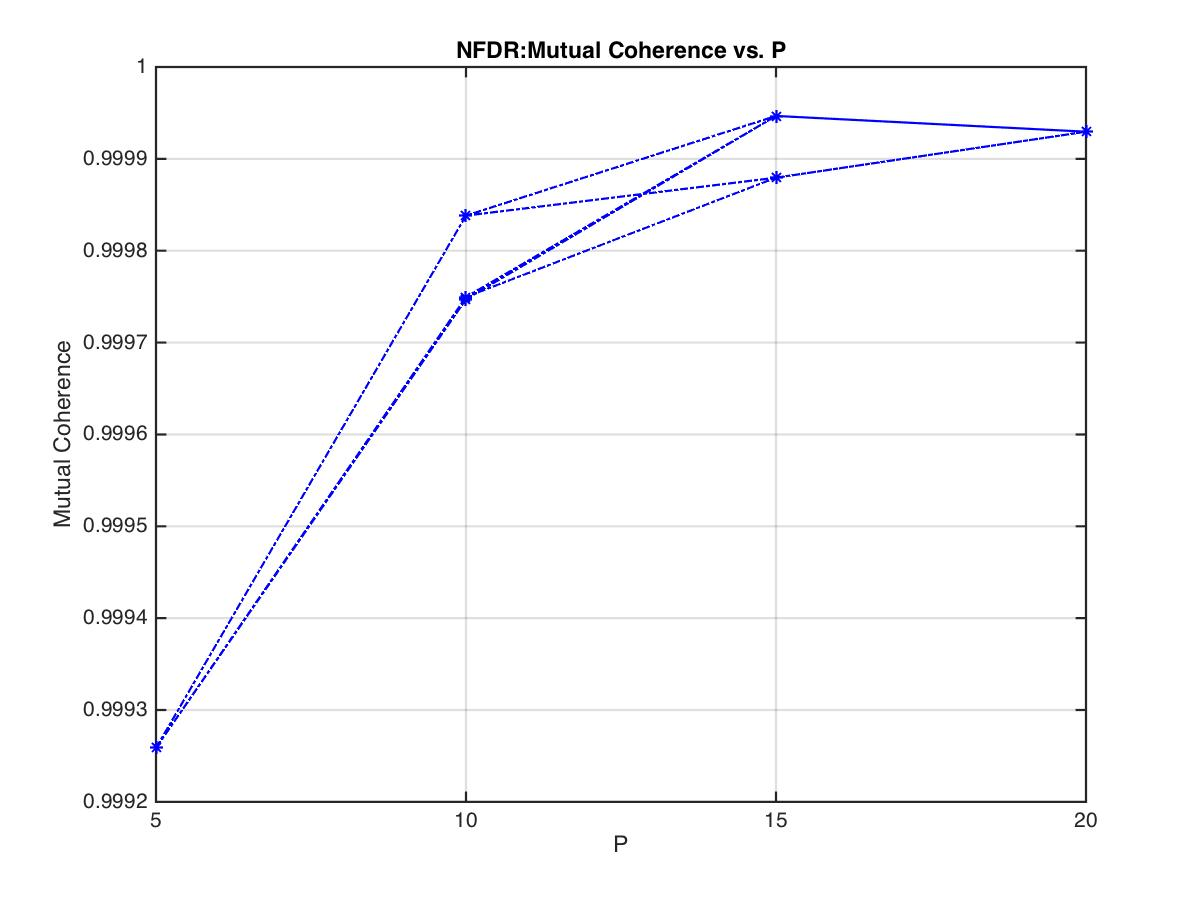
\includegraphics[width=4cm,center]{NFDR_Mutual_Coherence}
        \\ NFDR MC vs. P
        \centering
    \end{column}
    \begin{column}{0.33\textwidth}
        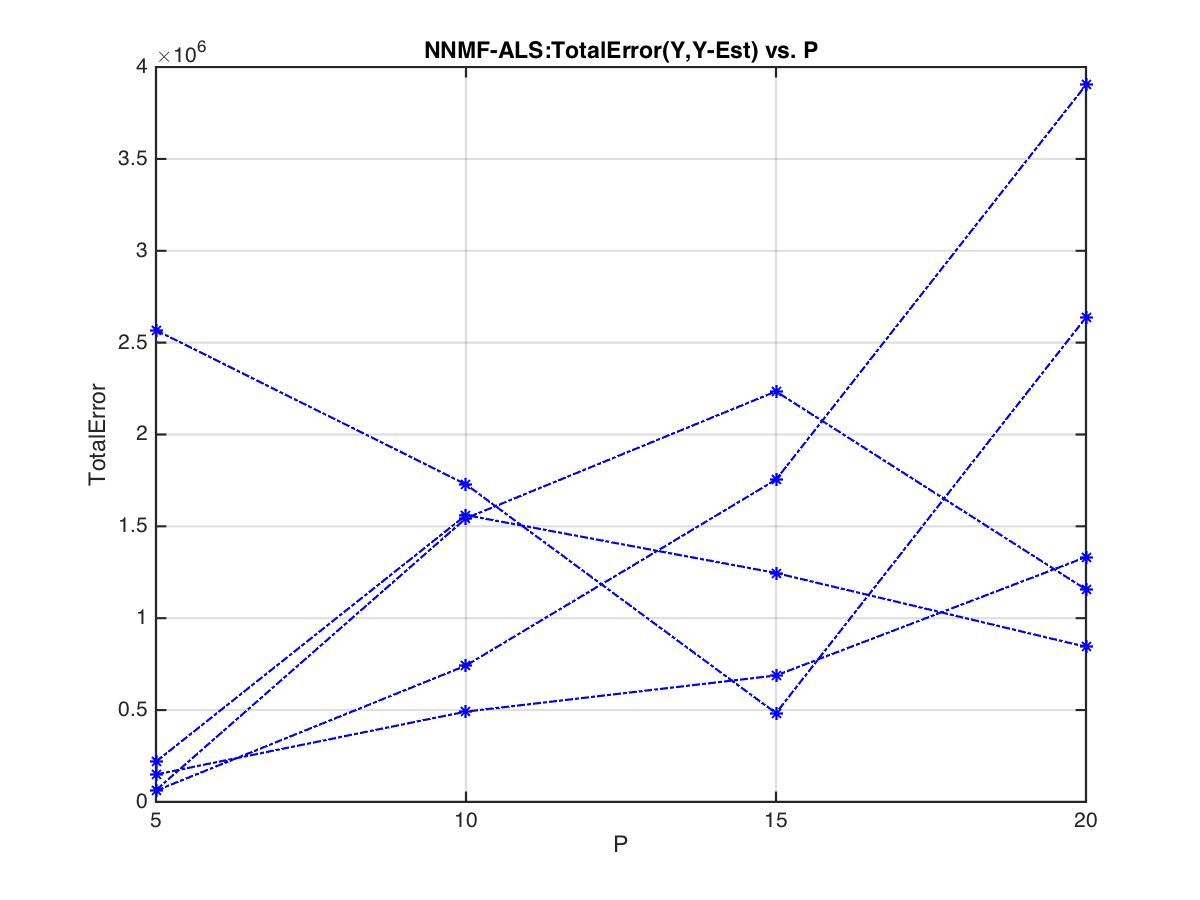
\includegraphics[width=4cm,center]{NNMF-ALS_TotalError}
        \\ ALS Error vs. P 
        \centering

        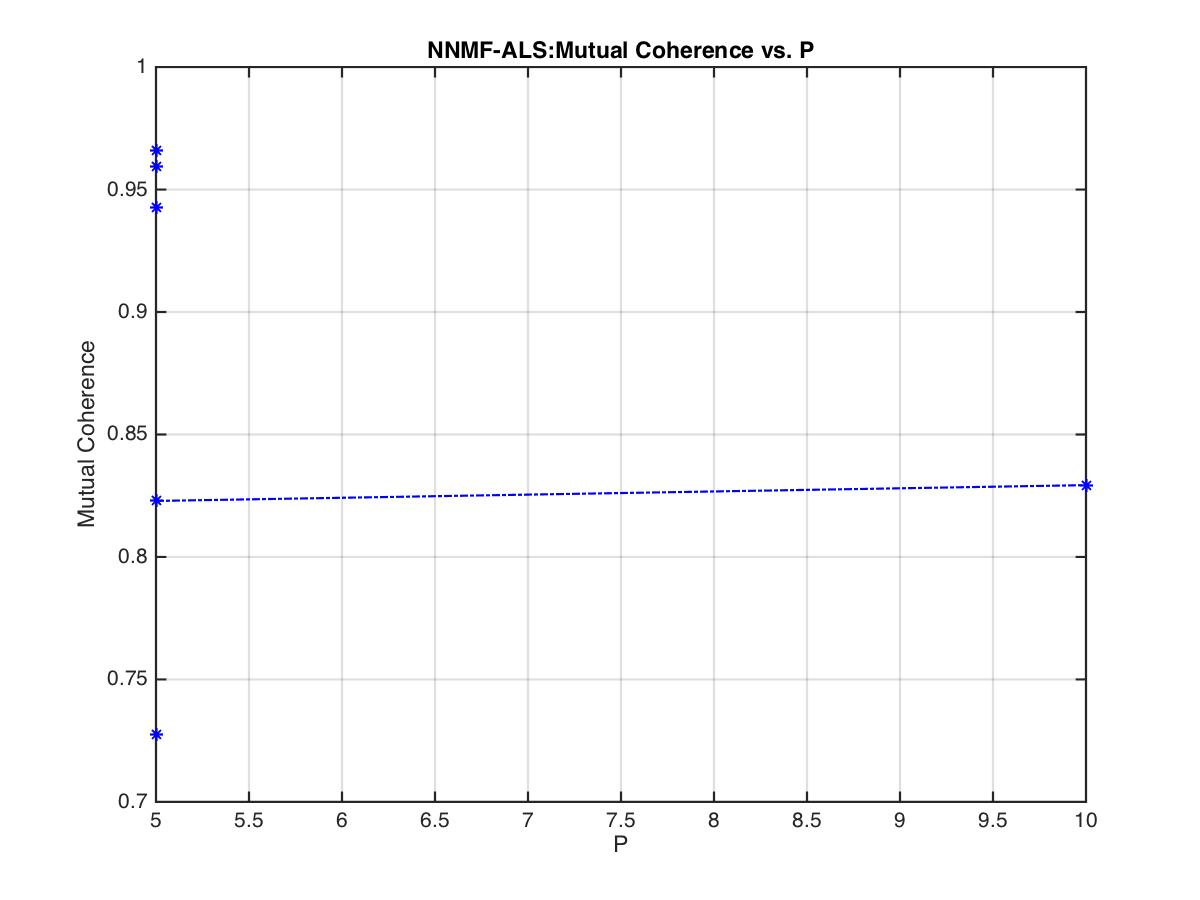
\includegraphics[width=4cm,center]{NNMF-ALS_Mutual_Coherence}
        \\ ALS MC vs. P
        \centering
    \end{column}
\end{columns}
\end{frame}

%------------------------------------------------
\begin{frame}
\frametitle{Numerical Error $\&$ Mutual Coherence}
\begin{columns}
    \begin{column}{0.33\textwidth}
        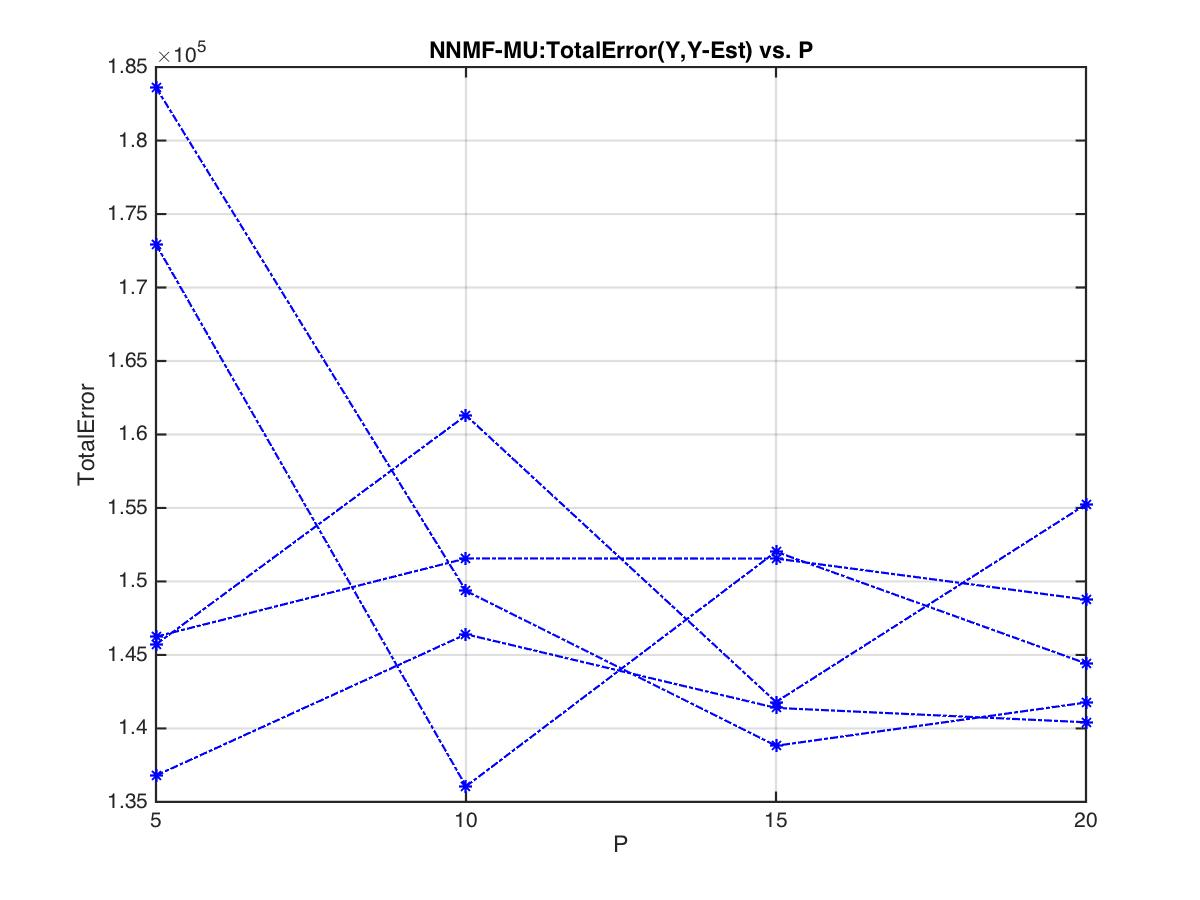
\includegraphics[width=4cm,center]{NNMF-MU_TotalError}
        \\ MU Error vs. P
        \centering

        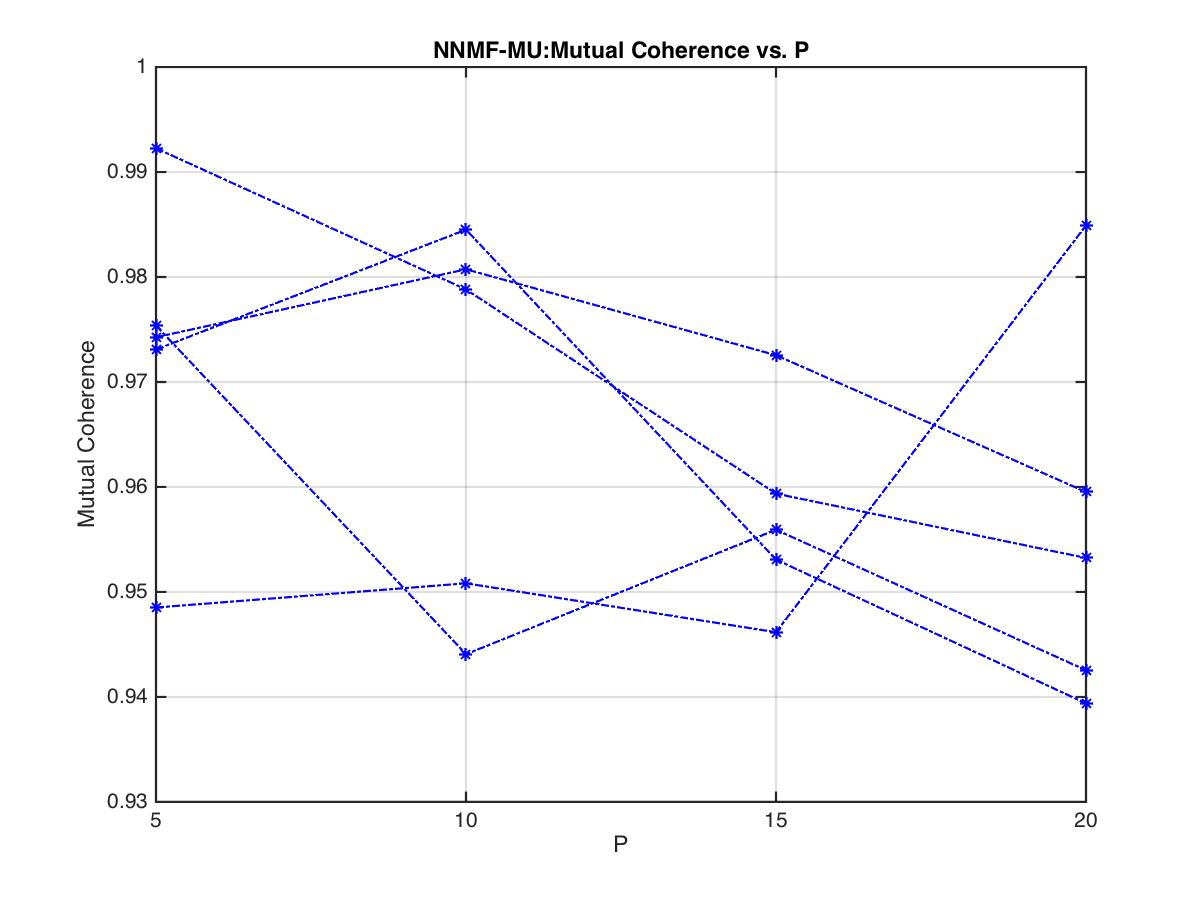
\includegraphics[width=4cm,center]{NNMF-MU_Mutual_Coherence}
        \\ MU MC vs. P
        \centering
    \end{column}
    \begin{column}{0.33\textwidth}
        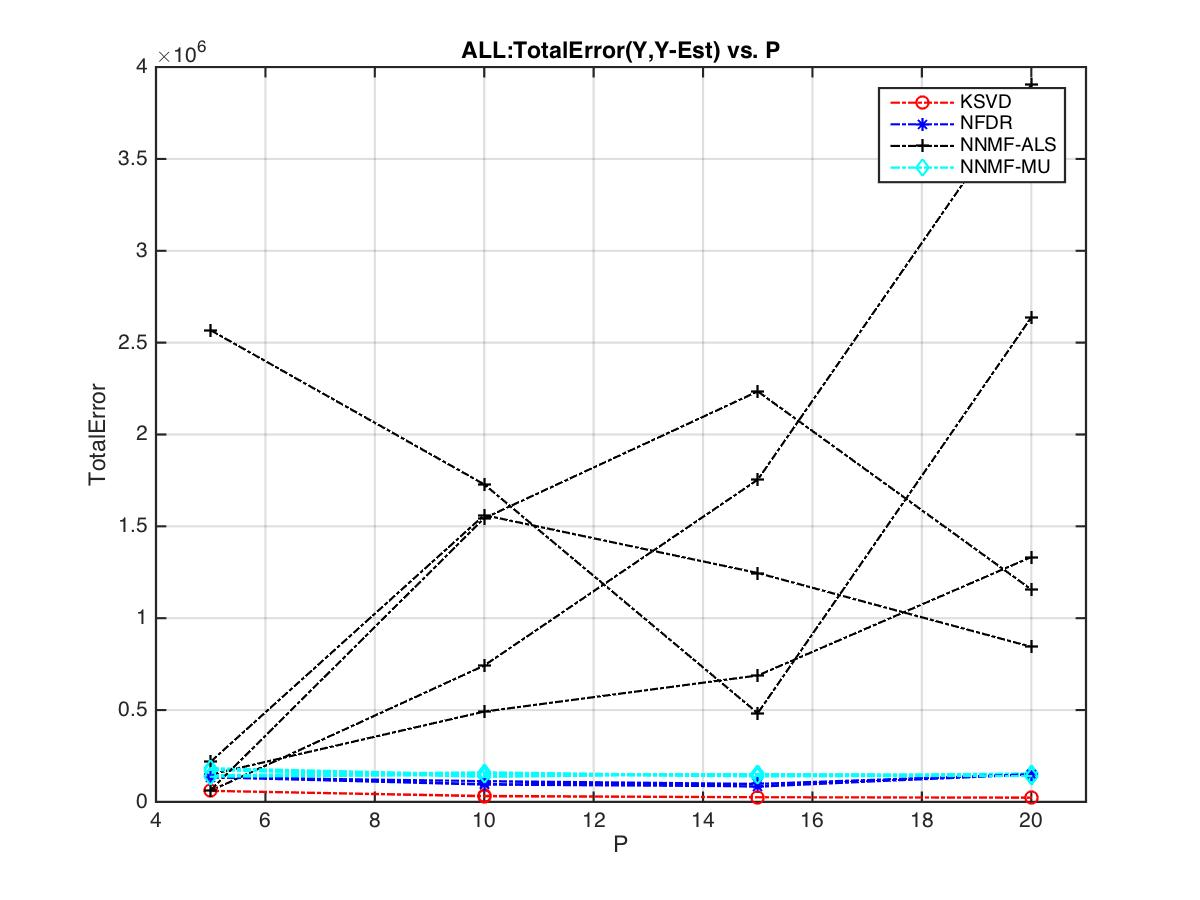
\includegraphics[width=4cm,center]{ALL_TotalError}
        \\ ALL Error vs. P
        \centering

        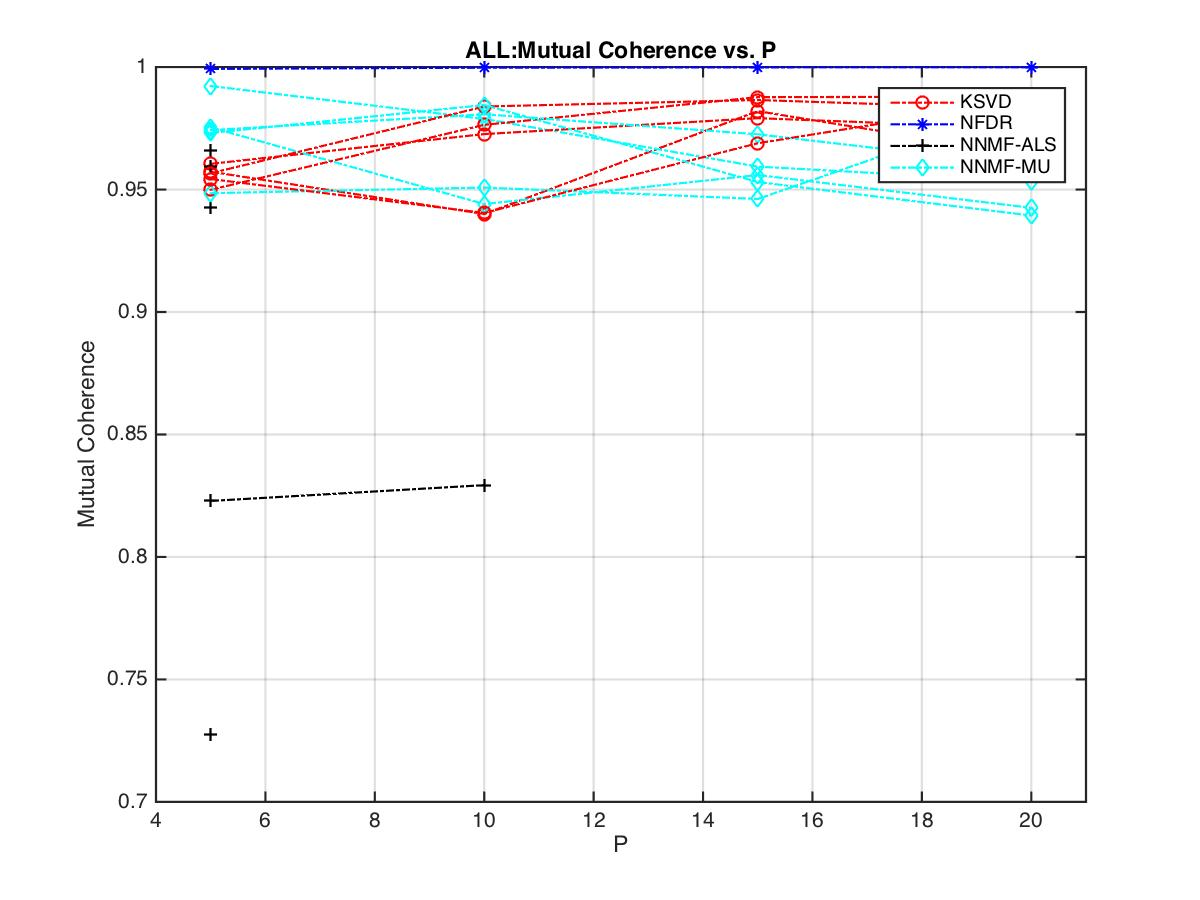
\includegraphics[width=4cm,center]{ALL_Mutual_Coherence}
        \\ ALL MC vs. P
        \centering
    \end{column}
    \begin{column}{0.33\textwidth}
        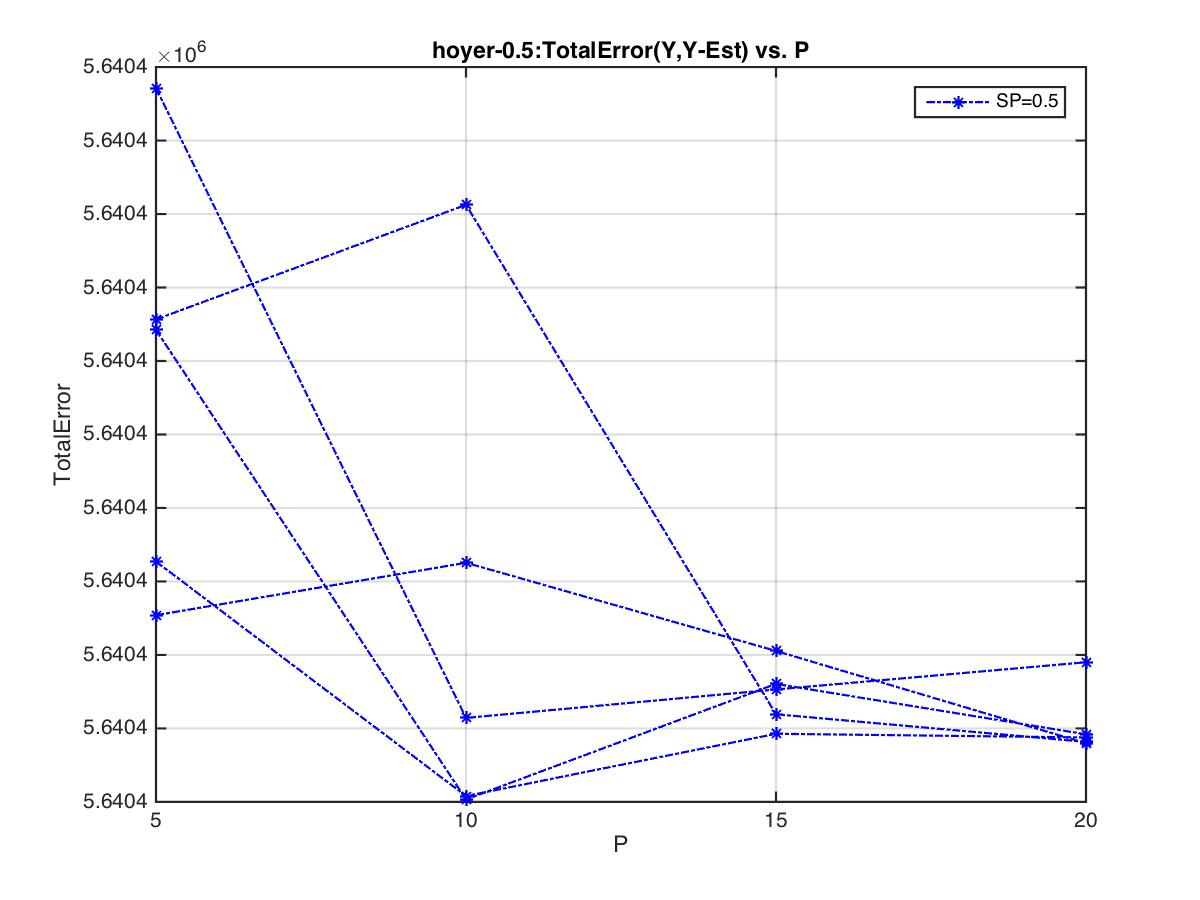
\includegraphics[width=4cm,center]{hoyer-05_TotalError}
        \\ Hoyer 0.5 Error vs. P 
        \centering

        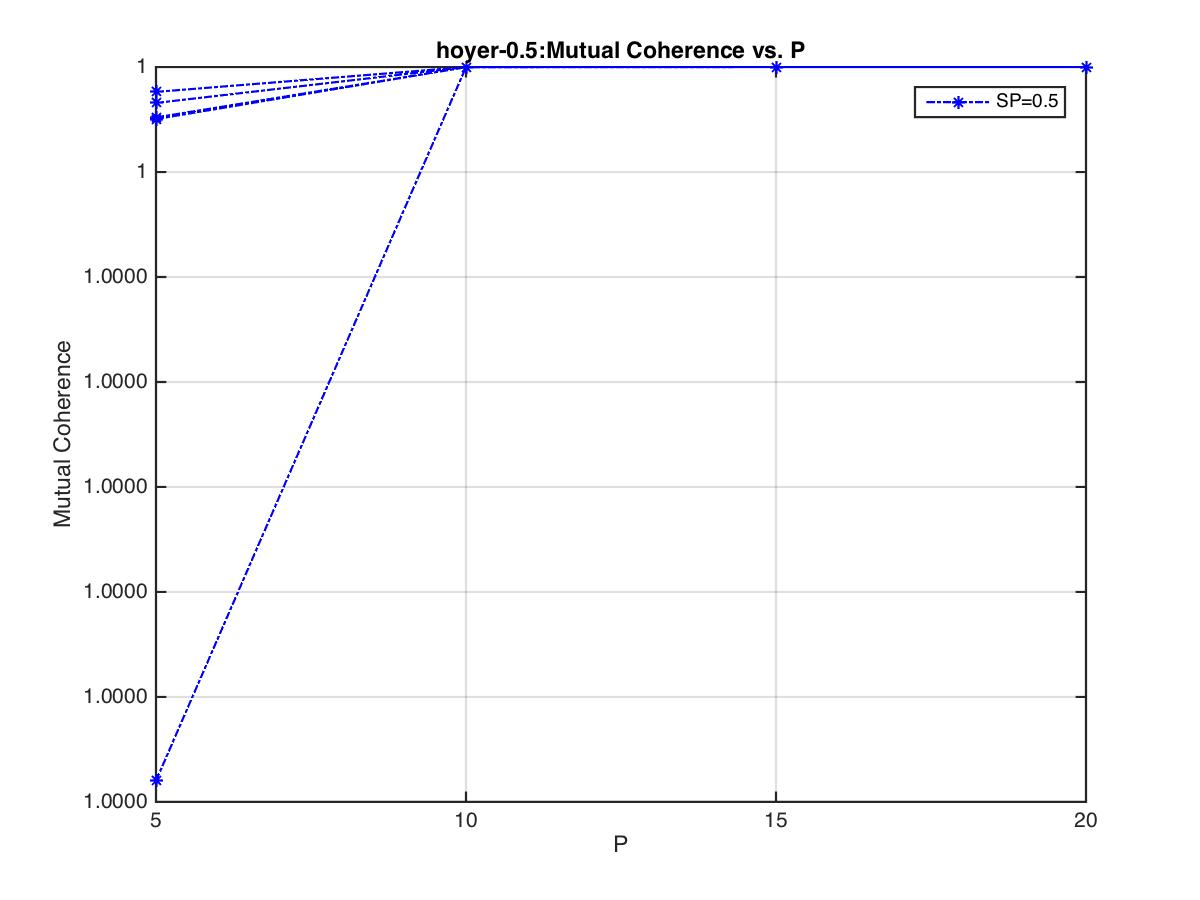
\includegraphics[width=4cm,center]{hoyer-05_Mutual_Coherence}
        \\ Hoyer 0.5 MC  vs. P
        \centering
    \end{column}
\end{columns}
\end{frame}

%------------------------------------------------
\begin{frame}
\frametitle{Numerical Error $\&$  Mutual Coherence}
\begin{columns}
    \begin{column}{0.33\textwidth}
        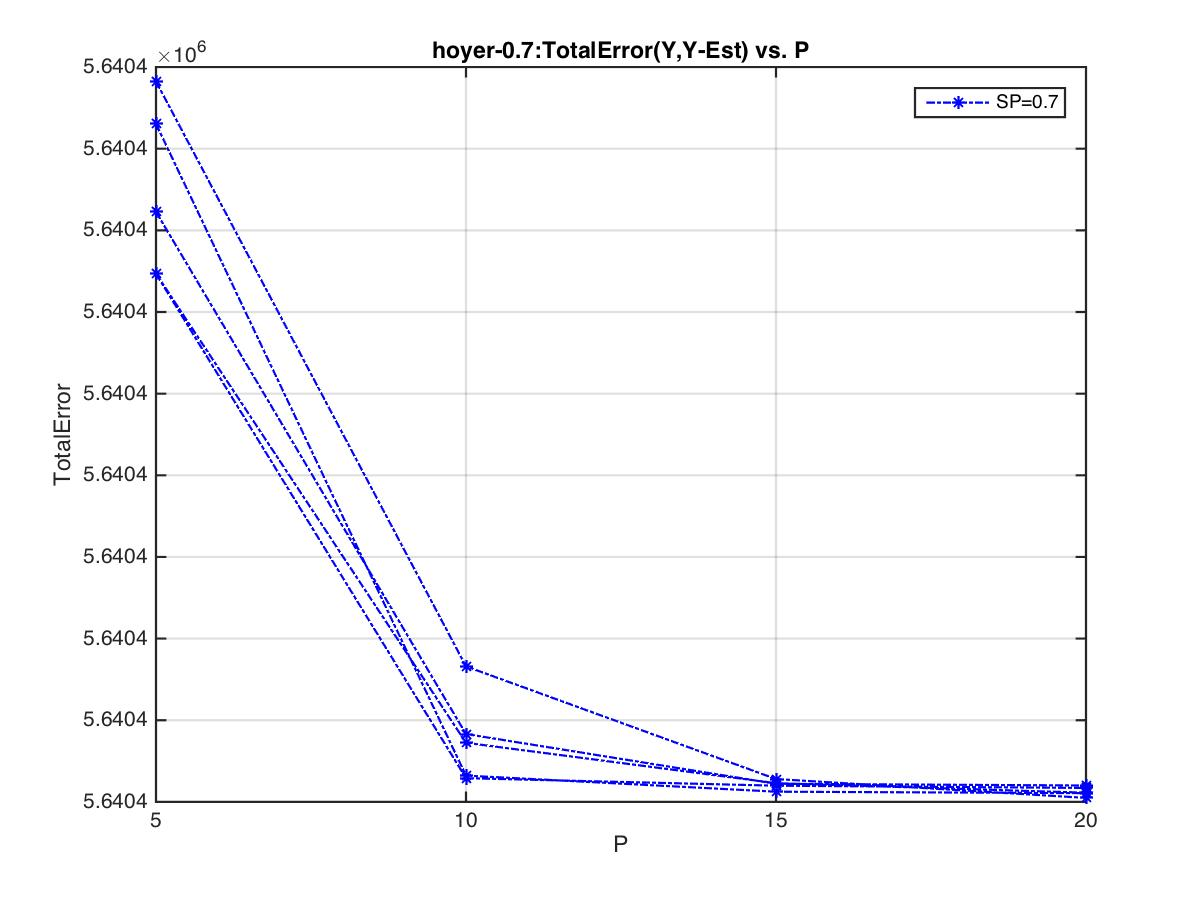
\includegraphics[width=4cm,center]{hoyer-07_TotalError}
        \\  Hoyer 0.7 Error vs. P 
        \centering

        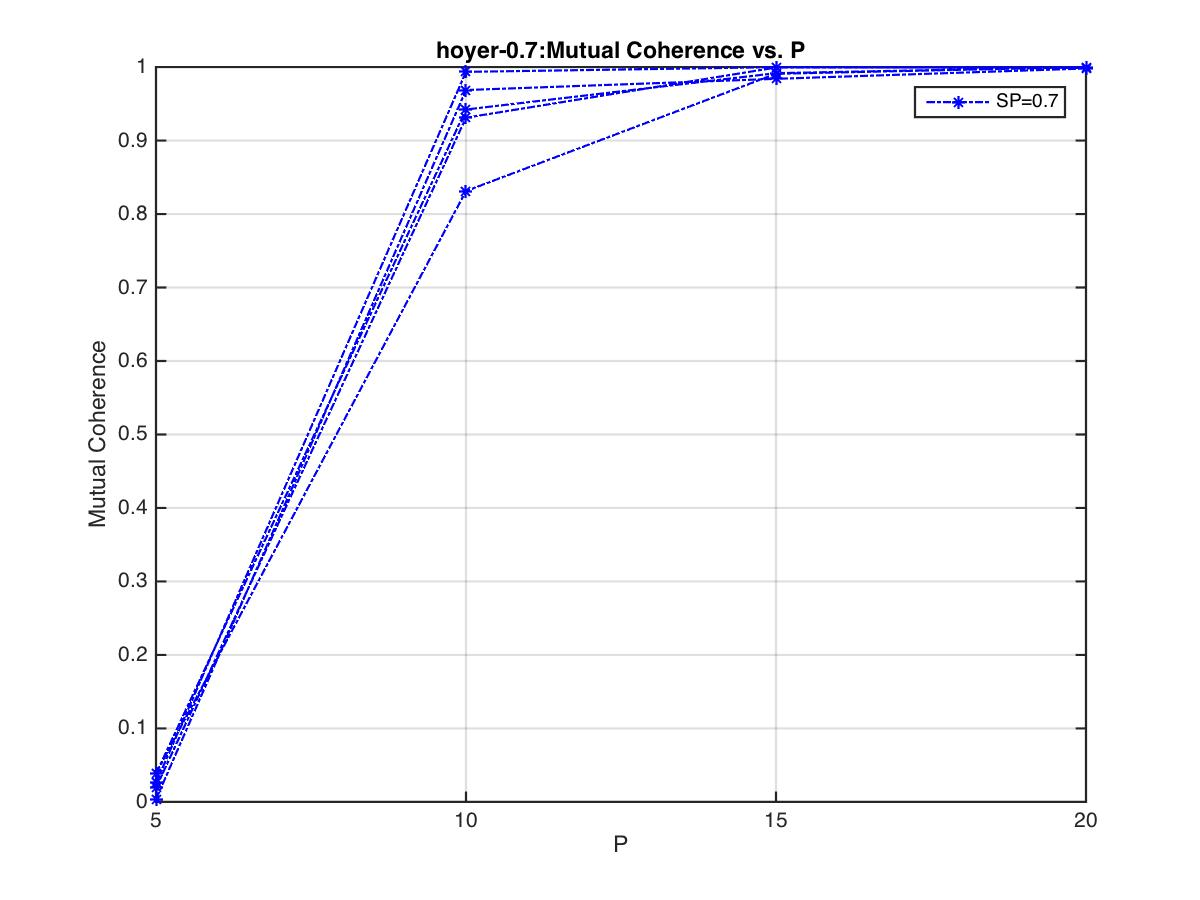
\includegraphics[width=4cm,center]{hoyer-07_Mutual_Coherence}
        \\  Hoyer 0.7 MC vs. P
        \centering
    \end{column}
    \begin{column}{0.33\textwidth}
        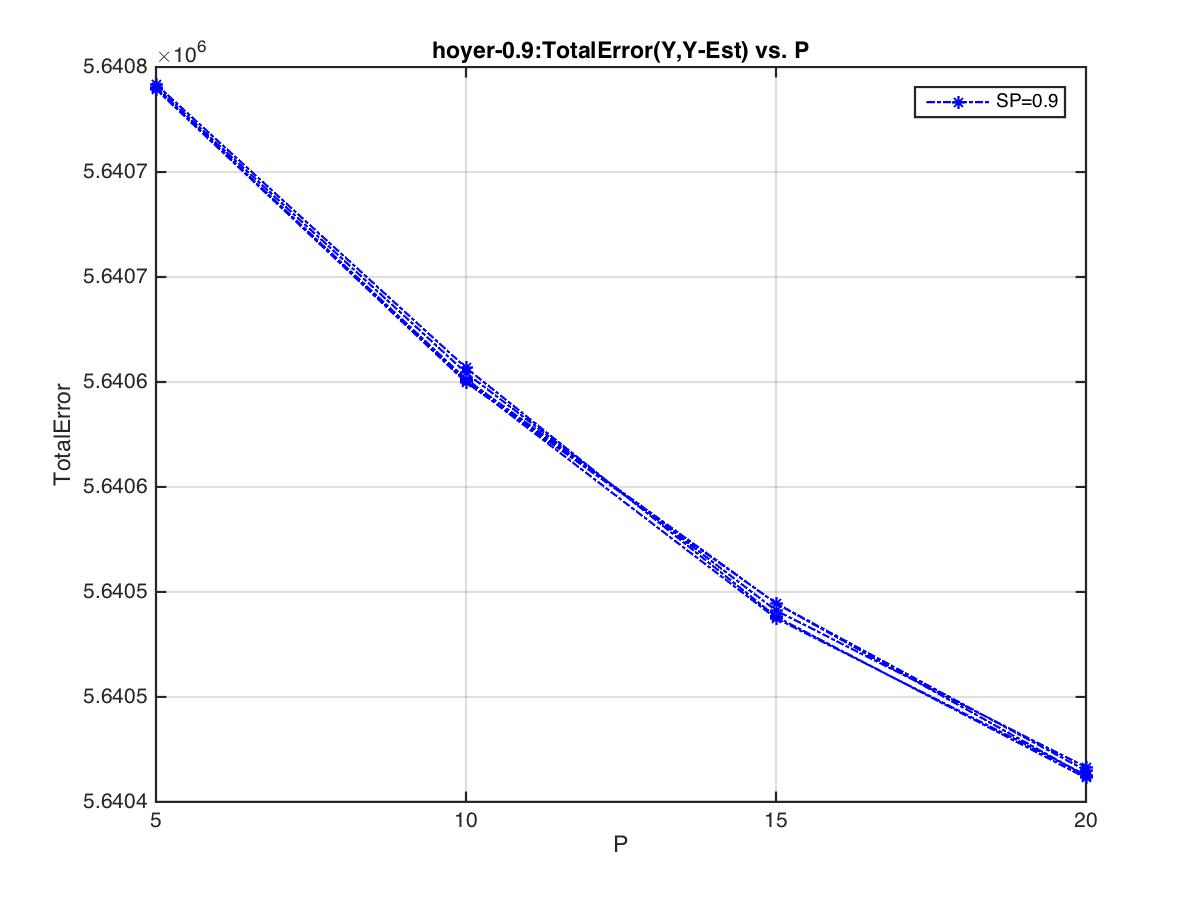
\includegraphics[width=4cm,center]{hoyer-09_TotalError}
        \\ Hoyer 0.9 Error vs. P 
        \centering

        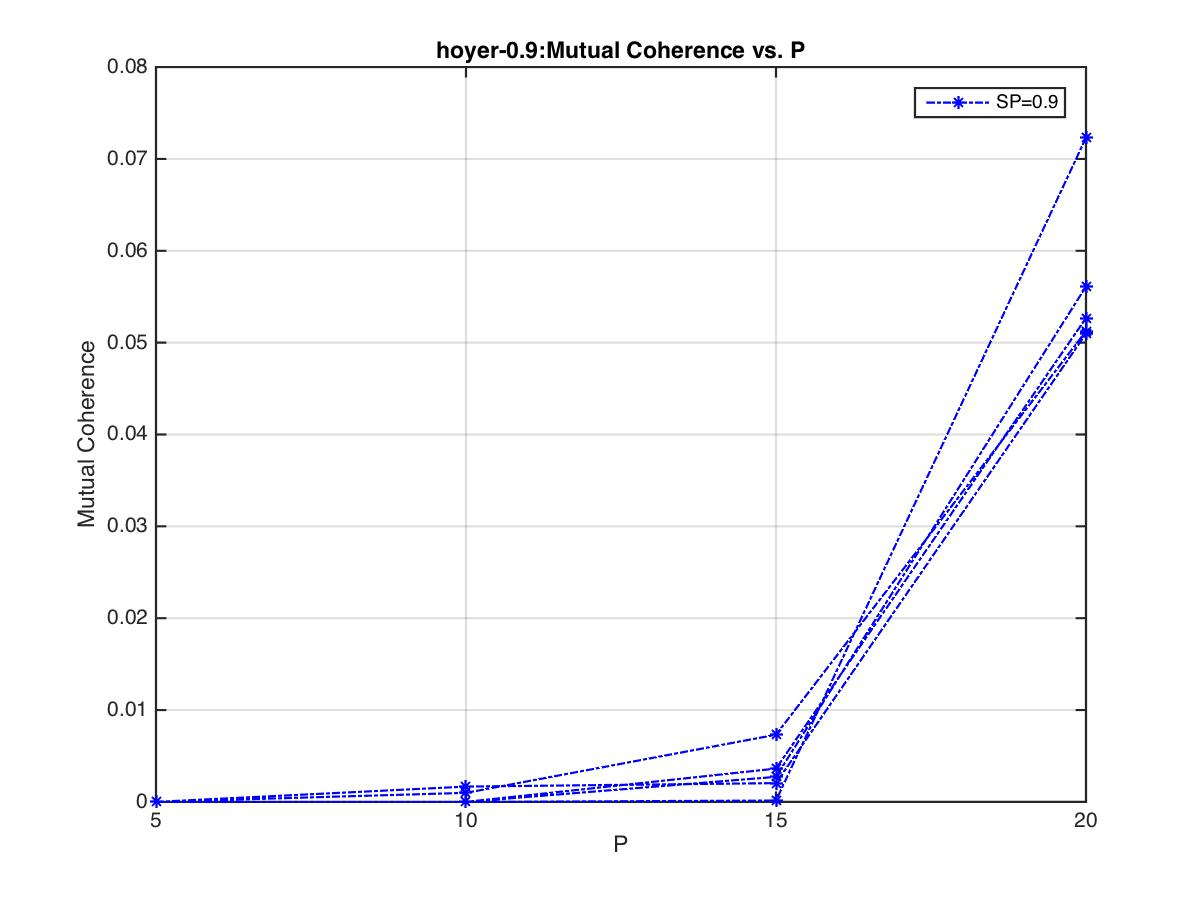
\includegraphics[width=4cm,center]{hoyer-09_Mutual_Coherence}
        \\ Hoyer 0.9 MC vs. P
        \centering
    \end{column}
    \begin{column}{0.33\textwidth}
        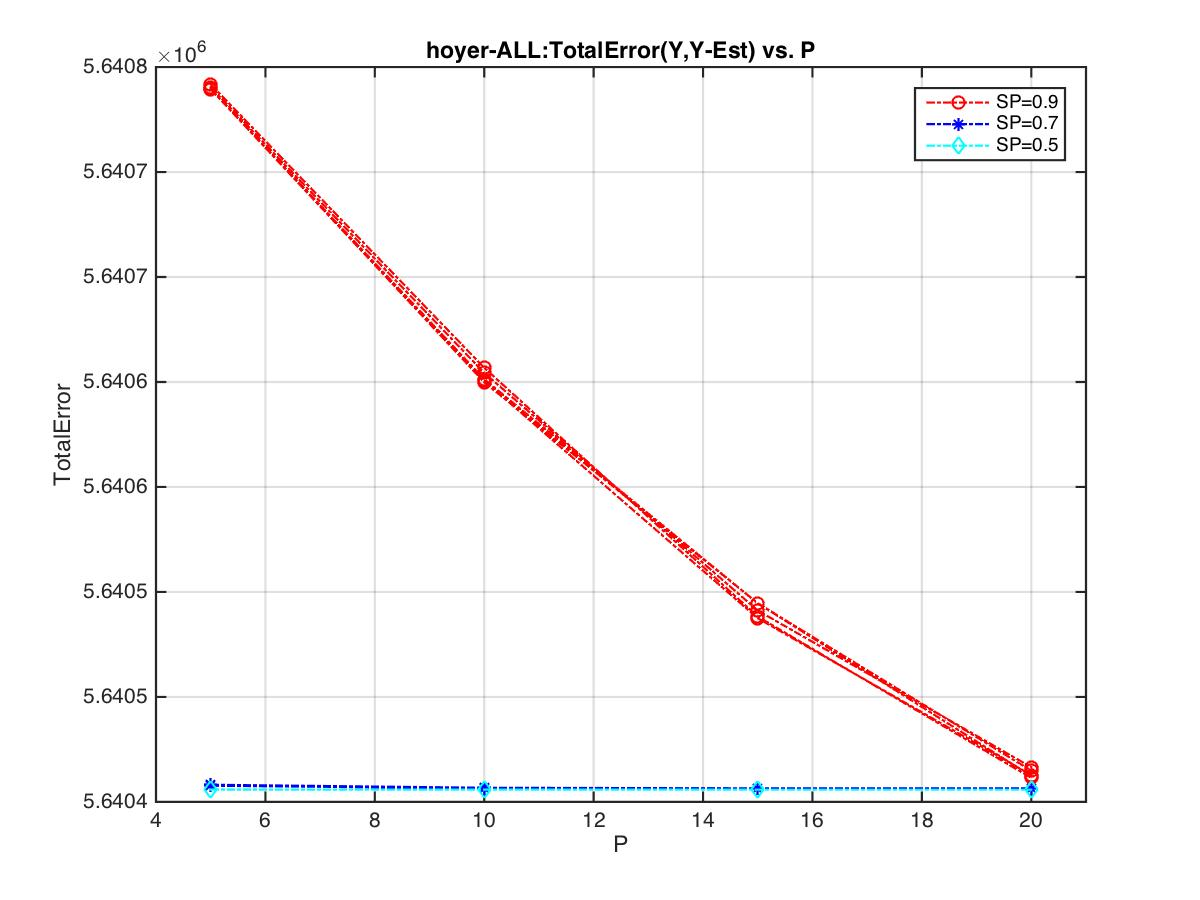
\includegraphics[width=4cm,center]{hoyer-ALL_TotalError}
        \\ Hoyer All Error vs. P 
        \centering

        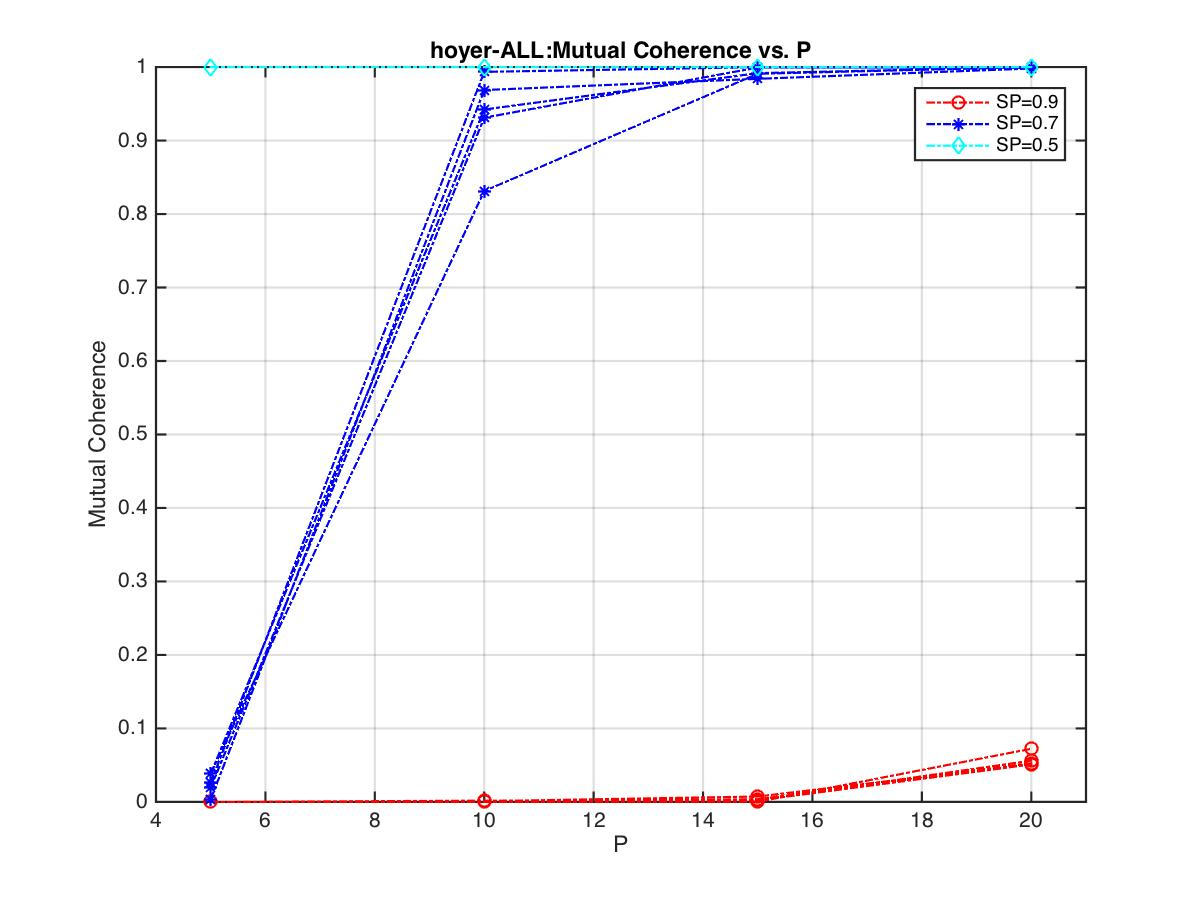
\includegraphics[width=4cm,center]{hoyer-ALL_Mutual_Coherence}
        \\ Hoyer All MC  vs. P
        \centering
    \end{column}
\end{columns}
\end{frame}

%------------------------------------------------

\begin{frame}
\frametitle{Reconstruction ALS and MU}
\begin{columns}
    \begin{column}{0.33\textwidth}
        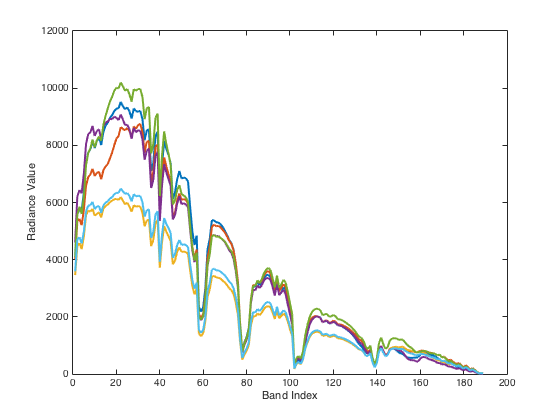
\includegraphics[width=4cm,center]{radiance}
        \\ Original Radiance Data
        \centering

        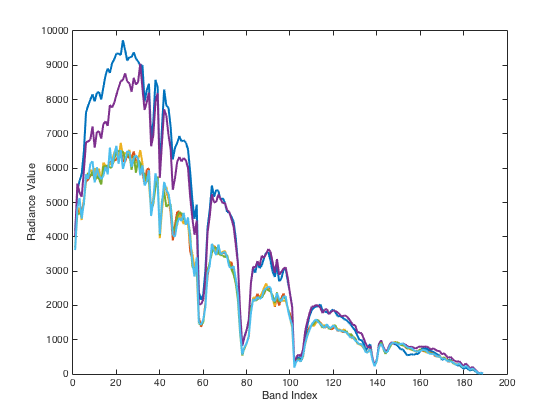
\includegraphics[width=4cm,center]{recon_nfindr}
        \\ NFINDR Result
        \centering
    \end{column}
    \begin{column}{0.33\textwidth}
        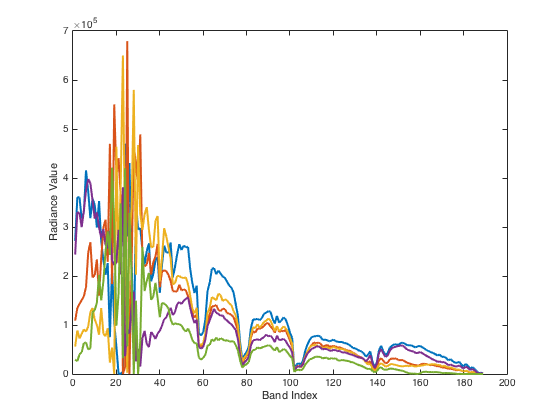
\includegraphics[width=4cm,center]{recon_als}
        \\ ALS Result
        \centering

        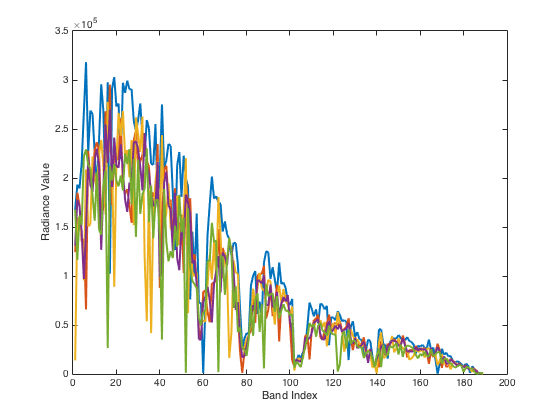
\includegraphics[width=4cm,center]{recon_mult}
        \\ Multiplicative Result
        \centering
    \end{column}
    \begin{column}{0.33\textwidth}
        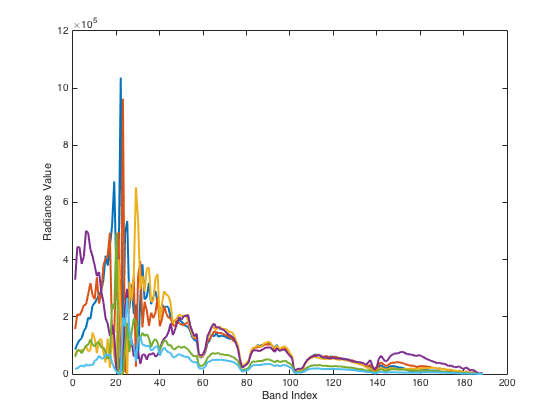
\includegraphics[width=4cm,center]{recon_mult_init_als}
        \\ ALS/Mult Result
        \centering

        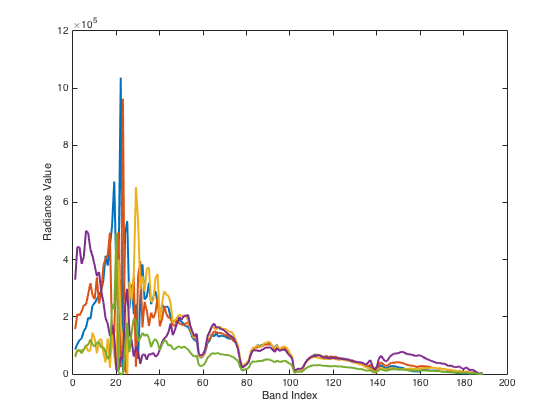
\includegraphics[width=4cm,center]{recon_asl_init_mult}
        \\ Mult/ALS Result
        \centering
    \end{column}
\end{columns}
\end{frame}

%------------------------------------------------
\begin{frame}
\frametitle{Reconstruction Hoyer and NN-KSVD}
\begin{columns}
    \begin{column}{0.33\textwidth}
        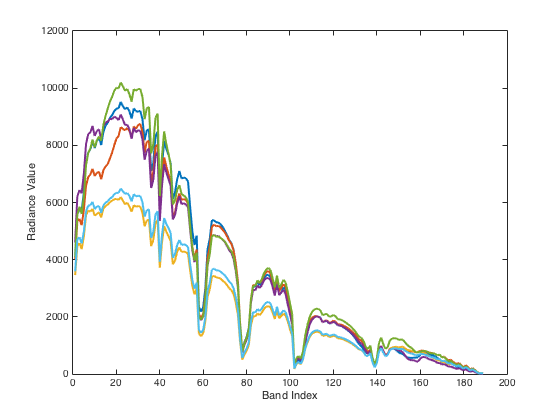
\includegraphics[width=4cm,center]{radiance}
        \\ Original Radiance Data
        \centering

        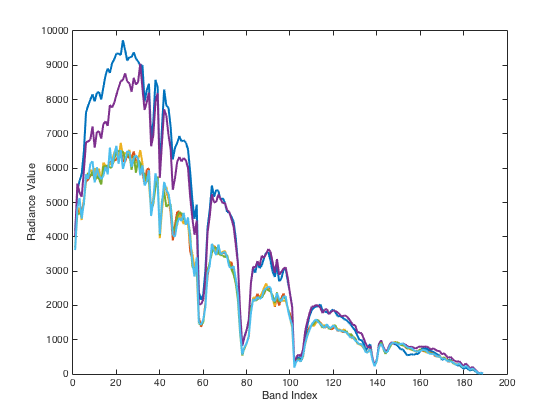
\includegraphics[width=4cm,center]{recon_nfindr}
        \\ NFINDR Result
        \centering
    \end{column}
    \begin{column}{0.33\textwidth}
        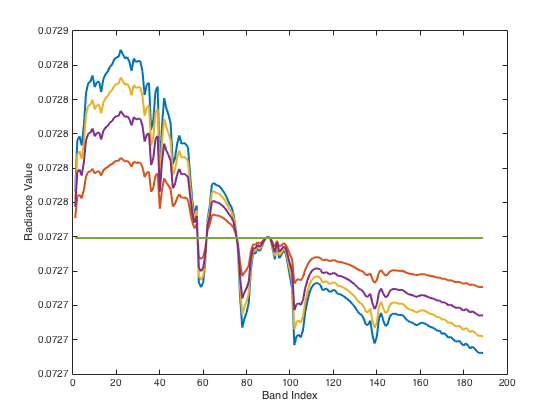
\includegraphics[width=4cm,center]{recon_hoyer_0_7}
        \\ Hoyer (Sparsity = 0.7)
        \centering

        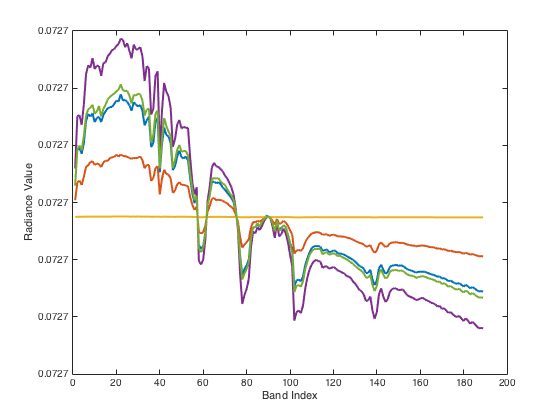
\includegraphics[width=4cm,center]{recon_hoyer_0_99}
        \\ Hoyer (Sparsity = 0.99)
        \centering
    \end{column}
    \begin{column}{0.33\textwidth}
        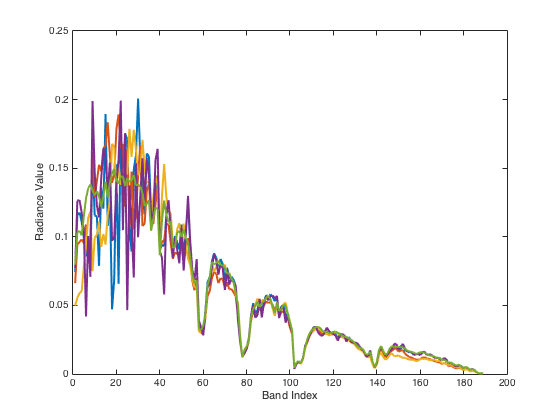
\includegraphics[width=4cm,center]{recon_ksvd_10iter}
        \\ KSVD 10 Iterations
        \centering

        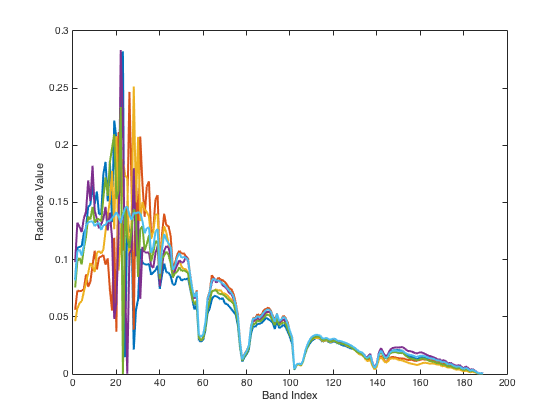
\includegraphics[width=4cm,center]{recon_ksvd_250iter}
        \\ KSVD 250 Iterations
        \centering
    \end{column}
\end{columns}

\end{frame}

%------------------------------------------------
\begin{frame}
\frametitle{Algorithm Rankings}

\begin{tabular}{| l || c | c | c | c | c |}
\hline
\bf{Criteria} & \bf{Best} & & & & \bf{Worst} \\
\hline
\hline
\bf{Abs Error} & KSVD & NFINDR & MU & ALS & Hoyer \\
\hline
\bf{Repeatability} & Hoyer & KSVD & NFINDR & MU & ALS \\
\hline
\bf{Increasing P} & KSVD & Hoyer & NFINDR & ALS & MU \\
\hline
\bf{Shape} & Hoyer & NFINDR & KSVD & ALS & MU \\
\hline
\bf{Run time} & ALS & MU & Hoyer & NFINDR & KSVD \\
\hline
\end{tabular}

\end{frame}

%------------------------------------------------
\begin{frame}
\frametitle{Conclusions}

\begin{itemize}
\item NMF can be used to do linear unmixing of HSI data into constituent materials
\item Scale and permutation ambiguity need application data to resolve
\item Sparsity helps considerably with the uniqueness and repeatability
    \begin{itemize}
        \item However, sparsity needs to be known a-priori
    \end{itemize}
\item Sparsity did resolve the shape better
    \begin{itemize}
        \item However, Hoyer frequently converged to a uniform answer
    \end{itemize}
\item The run time of KSVD was much larger than the other algorithms
\end{itemize}

\end{frame}

%------------------------------------------------
\begin{frame}
\frametitle{References}
\footnotesize{
\begin{thebibliography}{99}

\bibitem[chang_2013]{p1} Chein-I Chang (2013)
\newblock Hyperspectral Data Processing: Algorithms Design and Analysis
\newblock \emph{Wiley}, Appendix A.4.2

\bibitem[cding_2005]{p1} Chris Ding, He Xiaofeng, Horst Simon (2005)
\newblock On the Equivalence of Nonnegative Matrix Factorization and Spectral Clustering
\newblock \emph{Proceedings of SIAM Data Mining Conference} 4, 606 -- 610.

\bibitem[cding_2008]{p1} Chris Ding, Li Tao, Peng Wei (April 2008)
\newblock On the Equivalence Between Non-negative Matrix Factorization and Probabilistic Latent Semantic Indexing
\newblock \emph{Computational Statistics and Data Analysis} 52.8, 3913 -- 3927.

\bibitem[Lee_1999]{p1} Daniel D. Lee, and H. Sebastian Seung (October 1999)
\newblock Learning the parts of objects by non-negative matrix factorization
\newblock \emph{Nature} 401, 788 -- 791.

\end{thebibliography}
}
\end{frame}

%------------------------------------------------
\begin{frame}
\frametitle{References}
\footnotesize{
\begin{thebibliography}{99}

\bibitem[Lee_2001]{p1} Daniel D. Lee, and H. Sebastian Seung
\newblock Algorithms for Non-negative Matrix Factorization
\newblock \emph{Advances in Neural Information Processing Systems} 556 -- 562.

\bibitem[bannon_2009]{p1} David Bannon (2009)
\newblock Hyperspectral Imaging: Cubes and Slices
\newblock \emph{Nature Photonic} 3, 627 - 629.

\bibitem[donoho_2003]{p1} David L. Donoho (March 2003)
\newblock Optimally Sparse Representation in General Dictionaries via L1 Minimization
\newblock \emph{Proceeds of the National Academy of Science} 100, 2197 -- 2202.

\bibitem[Guoxu_2014]{p1} Guoxu Zhou, Andrzej Cichocki, Qibin Zhao, and Shengli Xie (May 2014)
\newblock Nonnegative Matrix and Tensor Factorizations
\newblock \emph{IEEE Signal Processing} 54(14).


\end{thebibliography}
}
\end{frame}

%------------------------------------------------
\begin{frame}
\frametitle{References}
\footnotesize{
\begin{thebibliography}{99}

\bibitem[ivana_2011]{p1} Ivana Tosic, Pascal Frossard (March 2011)
\newblock Dictionary Learning, What is the right representation for my signal?
\newblock \emph{IEEE Signal Processing Magazine} March 2011, 27 -- 38.

\bibitem[Aharon_2006]{p1} Michal Aharon, Michael Elad, Alfred Bruckstein (November 2006)
\newblock K-SVD: An Algorithm for Designing Overcomplete Dictionaries for Sparse Representation
\newblock \emph{IEEE Trans. on Signal Processing} Vol. 54, No. 11, 4311 -- 4322.

\bibitem[elad_2006]{p1} Michal Aharon and Michael Elad (2006)
\newblock \emph{https://github.com/jbhuang0604/SelfSimSR/tree/master/Lib/KSVD}

\bibitem[lopez_2013]{p1} Miles Lopes (2013)
\newblock Estimating unknown sparsity in compressed sensing
\newblock \emph{International Conf. on Machine Learning (ICML)} arXiv:1204.4227.

\end{thebibliography}
}
\end{frame}

%------------------------------------------------
\begin{frame}
\frametitle{References}
\footnotesize{
\begin{thebibliography}{99}

\bibitem[lopez_2015]{p1} Miles Lopes (2015)
\newblock Compressed Sensing without Sparsity Assumption
\newblock \emph{http://arxiv.org/abs/1507.07094} arXiv:1507.07094.

\bibitem[Mandula]{p1} Ondrej Mandula (2011)
\newblock \emph{https://github.com/aludnam/MATLAB/tree/master/nmfpack}

\bibitem[Hoyer_2002]{p1} Patrik Hoyer (February 2002)
\newblock Non-negative Sparse Coding
\newblock \emph{Neural Networks for Signal Processing} 12, 557 -- 565.

\bibitem[Hoyer_2004]{p1} Patrik Hoyer (November 2004)
\newblock Non-negative Matrix Factorization with Sparseness Constraints
\newblock \emph{Machine Learning Research} 5, 1457 -- 1469.

\bibitem[paatero_1994]{p1} Pentti Paatero, Unto Tapper (June 1994)
\newblock Positive Matrix Factorization: A non-negative factor model with optimal utilization of error estimates of data values
\newblock \emph{Environmetrics} 5(2), 111 -- 126.

\end{thebibliography}
}
\end{frame}

%------------------------------------------------

\end{document} 
